% This example An LaTeX document showing how to use the l3proj class to
% write your report. Use pdflatex and bibtex to process the file, creating 
% a PDF file as output (there is no need to use dvips when using pdflatex).

% Modified 

\documentclass{l3proj}
\usepackage{algorithm2e}
\usepackage{graphicx}
\usepackage{float}
\usepackage{caption}
\usepackage{subcaption}
\usepackage{url}
\begin{document}
\title{Project Title}
\author{Michael Kilian -- 1003819K \\
        Tony Lau -- 1102266L\\
        Dan Tomosoiu --1102486T \\
        Hector Grebbell -- 1007414G \\
        Peeranat Fupongsiripan -- 2056647F}
\date{19 March 2013}
\maketitle

\begin{abstract}
It is acknowledged that the cost of 
running evacuation drills in pubilc environments is relatively high both in time and money. This is because very often, the 
evacuation drills have to be run at night where the chosen environment is not in service and consequently additional payments for 
equipments, hiring evacuees and fire consultant are needed. This results in fewer number of evacuation drills. 
There are also some types of evacuation that cannot be drilled both safely and accurately such as a large fire.
An evacuation simulator is a possible solution to these problems which uses human behaviour in evacuation environment 
to predict the egress of a population. The aim of this project involves producing a three dimensions visualised 
evacuation simulator at The Tall Ship at Riverside, Glasgow. Not only focussing on implementation side, the research 
side is essentially indispensable. Psychology of mass emergency evacuation behaviour and crowd patterns are applied in 
order to best determine how people will react in an evacuation situation. Moreover, several path finding algorithms 
are studied to find out which one is suitable for the project.
The implementation side of this project 
involves the modelling of the chosen environment in 3D visualisation and simulating an evacuation on this model.
With this combination, evacuation simulator is more realistic.
\end{abstract}

\educationalconsent
\tableofcontents
%==============================================================================
\chapter{Introduction}
\label{introduction}

%\documentclass[a4paper,10pt]{article}
%\usepackage[utf8]{inputenc}
%\usepackage{graphicx}
%\usepackage{url}

%opening
%\title{Evacuation Simulator}
%\author{Team L}

%\begin{document}

%\maketitle

%\begin{abstract}
%It is acknowledged that the cost of 
%running evacuation drills in pubilc environments is relatively high both in time and money. This is because very often, the 
%evacuation drills have to be run at night where the chosen environment is not in service and consequently additional payments for 
%equipments, hiring evacuees and fire consultant are needed. This results in fewer number of evacuation drills. 
%There are also some types of evacuation that cannot be drilled both safely and accurately such as a large fire.
%An evacuation simulator is a possible solution to these problems which uses human behaviour in evacuation environment 
%to predict the egress of a population. The aim of this project involves producing a three dimensions visualised 
%evacuation simulator at The Tall Ship at Riverside, Glasgow. Not only focussing on implementation side, the research 
%side is essentially indispensable. Psychology of mass emergency evacuation behaviour and crowd patterns are applied in 
%order to best determine how people will react in an evacuation situation. Moreover, several path finding algorithms 
%are studied to find out which one is suitable for the project.
%The implementation side of this project 
%involves the modelling of the chosen environment in 3D visualisation and simulating an evacuation on this model.
%With this combination, evacuation simulator is more realistic.
%\end{abstract}
%
%\tableofcontents

\section{Introduction}

\subsection{Motivation}
Fatalities and injuries may be due to not only the nature of the disaster or emergency itself - whether a fire, 
bombing, sinking ship, or train or plane crash - but also human factors(behaviour of the evacuating crowd)~\cite[Section 1.1]{psychology}. These human factors include not only 
the effectiveness and appropriateness of emergency procedures and services, but also the behaviour of the evacuating crowd,
which has often been blamed for panic, disorganized, over-emotional, irrational and ineffective egress~\cite[Section 1.2]{psychology}. 
Other human factors which may play a role include decision-making~\cite[Section 2.2]{psychology} and the interpretation of events~\cite[Section 2.3]{psychology}
, leadership and social influence~\cite[Section 2.9]{psychology}, 
and after-care policies and practices~\cite[Section 3: Social Identity]{psychology}.Therefore, building an evaucation simulator which corresponds to the behaviour 
of evacuating crowd might help reduce fatalities and injuries within less time and budget.

\subsection{Definition of an Evacuation Simulator}
An evacuation simulator can be defined as a system to determine evacuation
times by predicting the egress of individuals in a building or similar
structure~\cite{evacuationSimulatordefinition}. They are used to identify
fication of weaknesses in the design of buildings which could detrimentally affect
the egress of persons in an evacuation and to aid personnel in
preparing for an evacuation~\cite{evacuationModel}.

\subsection{Why Implement an Evacuation Simulator}
The task of testing a building's evacuation procedure can be
both difficult and expensive. One approach is to hire members of the public
as stand-in ``evacuees'' and run a mock evaluation, such as those performed as part of Forward Defensive
in preparation for the London 2012 Olympics \cite{DailyMailEvacuation}. In theory this would allow an 
appropriate expert such as a consultant from a local fire department to assess the effectiveness
of an existing plan. However such tests on public buildings can be very expensive: the cost
of hiring evacuees could be significant. Also certain aspects of evacuations, such
as testing the possibility of a crush, can expose participants
to real danger. Finally if an evacuee knows they are participating in an experiment
their behaviour is inherently different than it would be in a real evacuation. This
phenomenon is known as Evaluation Apprehension\cite{EvalApprehension}.\\
For these reasons large scale tests on a building are rarely performed.
What a simulator provides is a means for an expert to extensively test the outcomes of evacuating a location
at minimal cost. By configuring variables in the simulation the expert can examine the probable outcome of multiple evacuations
and look for potential sources of danger in a building or evacuation procedure.

\subsection{Aims}
The Evacuation Simulation project’s aims are building a visual simulator that
can be used on a wide range of structures, for which models can be imported in
the final software without requiring extensive knowledge of the coding process.
Once the software is available to fire wardens or other authorities in charge of
building safety, they can cheaply run computer simulations on buildings and,
depending on the results provided, identify areas where improvements can be
made. Such improvements could be supplementing fire personel and/or fire
extinguishing equipment, opening alternative evacuation routes,
informing the intervening fire brigade of any areas with low evacuation rates etc.
This project intends to simulate an evacuation of The Tall Ship at Riverside(reasons why choosing the environment are explained in section 2),
Glasgow, in a virtual 3D environment. 
Specifically, the evacuation simulator is
expected to be able to accurately model the behaviour of people as they egress
from the ship and provide an interactive graphical user interface which gives
real-time feedback on the current state of all passengers.
It was decided to work towards an evacuation of the ship where the cause is
fire. This will require the exploration of various models of fire~\cite{fireEvacuationProcedure} and the challenge
of integrating it into the final evacuation system. It will also allow us to explore
the impact of smoke on the subjects within the ship.
The aim of this project is to produce a product which gives a
reasonably accurate representation of the egress of people which can hopefully
aid The Tall Ship in planning for an evacuation. The finished product can be
extended to include extra features, such as an enhanced fire model, to make the
simulation more realistic.

\subsubsection{A Multi-Agent Model of Individuals and Individual Behaviour}
Previous projects have emphasised crowd behaviour: they have modelled the population from a top down 
perspective with little consideration for the perception and interaction which an individual experiences in an evacuation.
One of the primary aims of this project is to represent a accurate model of individual behaviour.
Previous work has shown that multi-agent systems can achieve this. By taking this approach "the full effects of diversity that exists among agents in their attributes and behaviours can be observed as it
gives rises to the behaviour of the system as a whole" \cite{AgentBasedTutorial}.

\subsubsection{An Update of the Technologies Used in Previous Projects}
Many previous works in this field have made use of software packages such as Java 3D; these are now unsupported and 
would be difficult to extend in the future.
These are discussed in the Implementation section.

\subsubsection{Use of Navigation Meshes in Environment Modelling}
A Navigation Mesh is a graph representation of an environment in terms of a set of convex polygons which describe the `walkable' surface of an environment. This design aids agents in finding paths through large areas, whilst avoiding static obstacles in the environment.
This technique has largely been pioneered in Gaming, but is equally applicable in this setting. The benefits of a navigation mesh, or 'navmesh' is that it allows agents to move 
freely compared to other techniques such as representing the environment using a grid. A navmesh is typically combined with the powerful path finding algorithm A* to 
optimise agent movement \cite{A*Review}.

\subsection{Prerequisites}
Where possible all technical concepts used within this paper will be clearly defined. However, To fully understand the remainder of this report, the reader should have at least
minimum knowledge in the following areas:
\begin{itemize}
 \item Object-Oriented programming concepts (preferably in Java)
 \item Concurrent programming concepts
 \item Pathfinding simulation and collision detectance/avoidance~\cite{gameProgramming}~\cite{collisionDetection}
 \item Herding, flocking behaviour and boids~\cite{HAndBoid}~\cite{Fbehavior}
 \item Human behavioural traits~\cite{HumanBehaviouralTraits}
 \item 3 Dimentional Vectors
\end{itemize}

\subsection{Previous Work}

\subsubsection{Fluid Based Systems}
These systems model crowd movement as if the crowd were a fluid \cite{WikipediaFluidMechanics}, using equations and principles taken from Physics. 
Exodus \cite{GaleaNumericalSimulation,GaleaMathModelling} is an example of such a system. There are drawbacks in such a style 
of simulator. Crowds "have a choice in their direction, they have no conservation of momentum and can stop and start at will" \cite{StillCrowdDynamics}. 
These concepts are not accounted for in fluid models, and so this style of simulator is limited to estimating the movement of a crowd as a whole without
considering individual interactions.

\subsubsection{Matrix or Grid Based Systems}
In a matrix or grid based system, the floor of the environment is represented by a series of adjacent nodes, often square or hexagonal in shape. Each 
cell can represent open areas, areas blocked by a static obstacle, exits, etc. This method is becoming less common, but two formerly well know examples are 
Egress and Pedroute. It was suggested that the existing matrix-based models suffer from the
difficulties of simulating crowd cross flow and concourses; furthermore, the
assumptions employed in these models are questionable when compared with field observations \cite{StillCrowdDynamics}.

\subsubsection{Emergent Agent Based Systems}
The final class of simulator we discuss here is the emergent (agent based) simulator. In this approach the system is composed of autonomous
and interacting ``agents''. Agents interact within an environment using a defined set of simple relationships. The benefit of this approach is the introduction
of \emph{emergent} behaviour: ``patterns, structures and behaviours emerge that were not explicitly programmed into the models, but arise as the 
result of agent interactions'' \cite{AgentBasedTutorial}.\\
The MASSEgress project developed at Stanford University is an ongoing effort to develop a framework for the development of such systems \cite{MultiAgentFramework}.
It has also led to the production of at least one prototype implementing this framework. 
This project has utilised a modified version of this framework for the integration
of agent behaviour. This is discussed further in the Research and Implementation sections.

\subsection{Background}
At present, previous works discussed in last section are obsolete, as they were designed to use Java3D~\cite{java3D},
an old and currently unsupported library. JMonkeyEngine~cite{jmonkey} was chosen as a
replacement 3D development engine for this project. This is an open source
tool and has an active community surrounding it, which could help with solving
eventual problems that might appear when using it.
While some of the previous projects have flaws that make them unusable for
simulation of large environments~\cite{glasgowUSimulator}, one the current project’s main purposes is
scalability - importing of reasonably large building models and, once imported,
executing simulation on the resulted logical structure in a reasonable time-frame.

\section{Environment}
The Glenlee, the tall ship, was built at the Bay Yard in Port Glasgow and was one of a group of 10 steel sailing vessels 
built to a standard design for the Glasgow shipping firm of Archibald Sterling and Co. Ltd. 
She is a three masted barque, with length 245 feet, beam 37.5 feet and depth 22.5 feet.
The Glenlee first took to the water as a bulk cargo carrier in 1896. She circumnavigated the globe four times
and survived passing through the fearsome storms of Cape Horn 15 times before 
being bought by the Spanish navy in 1922 and being turned into a sail training vessel. 
The ship was modified and served in that role until 1969. She then operated as a training school until 1981 
when she was laid up in Seville Harbour and largely forgotten.
Nowadays, she is permanently docked at the Riverside Museum in Glasgow which operates a programme of year-round maritime 
themed events and activities, with specially devised talks and tours, school visits and costumed volunteer days.

\begin{center}
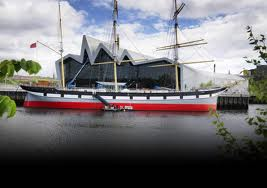
\includegraphics{../images/glasgowTallShip.jpg}
\\Figure 1: Glasgow Tall Shap
\end{center}
Current work on the project is based on evacuating The Tall Ship because 
\begin{itemize}
 \item It serves as both a tourist attraction and a function hall below decks.
 \item The ship is permanently docked and can be considered a static structure.
 \item Events can host up to 200 guests, excluding staff.
 \item It has a sufficiently complex structure in which to explore simulation techniques.
 \item No full scale evacuations have ever been held before - only staff have been used.
 \item These drills are infrequent.
\end{itemize}

\begin{center}
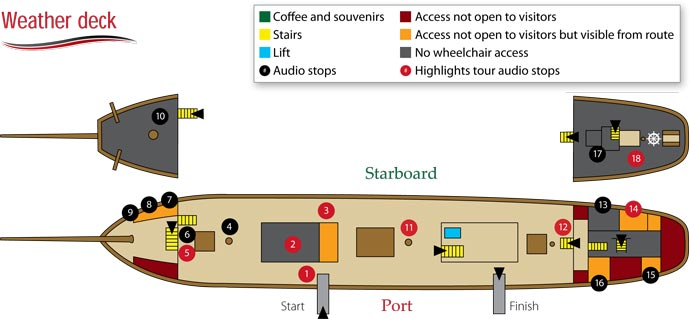
\includegraphics[scale=0.4]{../images/weatherdeck.jpg}
\\Figure 2: Weather Deck
\end{center}

\begin{center}
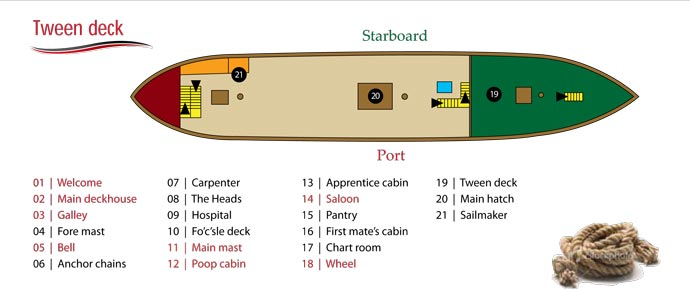
\includegraphics[scale=0.4]{../images/tweendeck.jpg}
\\Figure 3: Tween Deck
\end{center}

\begin{center}
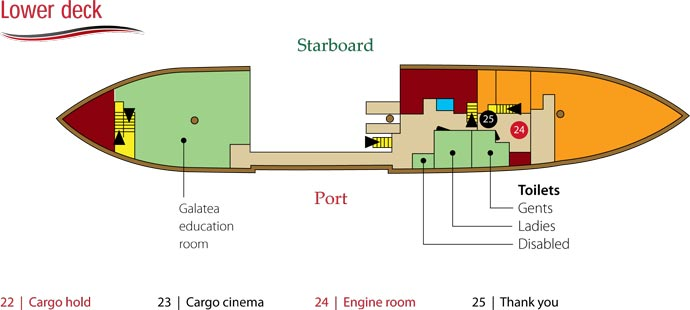
\includegraphics[scale=0.4]{../images/lowerdeck.jpg}
\\Figure 4: Lower Deck
\end{center}

\begin{center}
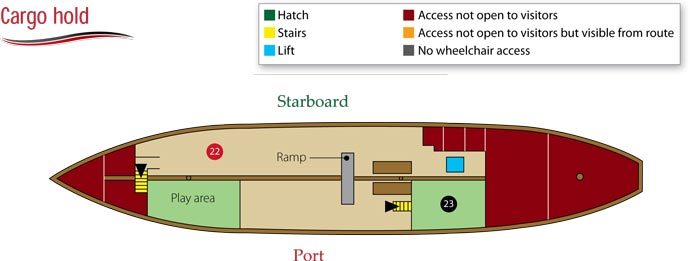
\includegraphics[scale=0.4]{../images/cargohold.jpg}
\\Figure 5: Cargo Hold
\end{center}

It is important to note that only small scale staff evacuations have been conducted on the ship
thus far considering the impractical nature of carrying out an evacuation with
actual visitors. Because of this restriction, an evacuation simulation of The
Tall Ship is ideal to assess the safety of visitors on the ship in the event of an
emergency evacuation.

%\bibliographystyle{unsrt}   % this means that the order of references
%			    % is dtermined by the order in which the
%			    % \cite and \nocite commands appear
%\bibliography{individual_ref}

%\end{document}

%\documentclass{article}
%\begin{document}

\section{Team Structure}
\label{Team:subsec:structure}
In order to develop a structured approach to task allocation, the software engineering tasks required were structured using the Administrative Programming Team \cite{AdministrativeProgrammingTeam}. This consists of the following roles:
\begin{itemize}
\item{\textbf{Project Manager} }
\item{\textbf{Librarian} }
\item{\textbf{Configuration Manager} }
\item{\textbf{Toolsmith} }
\item{\textbf{Quality Assuror}}
\end{itemize}

It should be emphasised that each person was not solely responsible for the tasks associated with their role; their responsibility is to coordinate these tasks within the team by proposing, implementing and maintaining effective procedures to achieve this.

In tandem with this, the team was further divided into two subteams for development:
\begin{itemize}
\item \textbf{Modelling and GUI Team:} responsible for development of any 3D models required including the final model of the ship. In the later stages of the project this team developed the graphical user interface.
\item \textbf{Core Implementation Team:} responsible for all other development tasks, including implementation of the navigation mesh, population model, etc.
\end{itemize}

By separating the development of the user interface from the development of the underlying program logic, the team aimed to promote a Model-View-Controller design. \cite[Ch 6.3.1]{SommervilleSoftwareEng}.
  
\section{Development Process}
\label{Team:subsec:process}
One of the challenges of designing an evacuation simulator is defining a level of accuracy which can be deemed acceptable with respect to the project's resources, and then translating this into an effective design which balances the use of up-to-date techniques with an implementation plan. Many of the techniques that this project aimed to implement are complex. These techniques are discussed further in the section \ref{research} Research.\\
Ultimately, it became clear that the most tangible way to make progress was to use a strategy of incremental prototyping \cite[Ch 2.3.2]{SommervilleSoftwareEng}. This would allow the team to progressively `scale up' ideas and to investigate the feasibility of implementing certain principles in a structured manner. However, incremental prototyping carries the following considerable risks which must be addressed:
\begin{itemize}
\item A tendency to produce low quality and difficult to maintain code.
\item Difficulties in managing change.
\item Tendency to sacrifice quality assurance and documentation because of poorly understood aims.
\end{itemize}

To mitigate these risks, several techniques taken from the field of agile development \cite[Ch. 3]{SommervilleSoftwareEng} were employed as follows:
\begin{itemize}
\item \textbf{Division into Subteams:} The team was divided as outlined above so as to allow these subteams to work in parallel on orthogonal tasks. This reduced communication overhead and the difficulty of managing change to the system.
\item \textbf{Constant Refactoring:} Before the completion of each prototype or upon fixing a defect, significant refactoring was undertaken to improve code quality.
\item \textbf{Pair Programming:} This technique was particularly helpful when fixing defects related to navigation (see Implementation \ref{implementation}) due to the complexity of these defects.
\item \textbf{Test First Development:} wherever the understanding of requirements was sufficient to allow it, test cases were developed for a feature before they were implemented.
\end{itemize}

%\end{document}


%==============================================================================
\chapter{Research}
\label{research}

\documentclass[a4paper,11pt]{article}
\usepackage[T1]{fontenc}
\usepackage[utf8]{inputenc}
\usepackage{lmodern}

\title{}
\author{}

\begin{document}
\section{Research into Human Behaviour}
\subsection{Non-adaptive Behaviour}
Adaptive behaviour is any behaviour is any behaviour ``which contributes directly or indirectly to an individuals survival''.
Conversely non-adaptive behaviour is any behaviour which may be counter productive to an individuals survival \cite{AdaptiveBehaviourWiki}.
In the context of an evacuation this refers to high risk actions which occur in a crowd such as stampede, pushing and shoving others,
trampling others, etc.\\
The introduction of non-adaptive behaviour can be connected to the stress a person is feeling. More specifically, Law et al \cite{CIFEResearchProposal} propose that there are three factors which contribute to the emergence of adaptive or non-adaptive behaviour:
\begin{itemize}
  \item{\textbf{Panic}: when a person perceives danger they are more likely to make irrational decisions based on instinct \cite{PanMASSEgressThesis}.}
  \item{\textbf{Decision-making}: although panicked, a person is still capable of making rational decisions. This increases the likelihood of the individual making adaptive choices, such as correctly recognising an exit or refraining from shoving upon exiting.}
  \item{\textbf{Levels of urgency to exit}: individuals within a group will experience varying levels of arguing to leave the environment based on the level of danger they perceive themselves to be in. High urgency causes individuals to behave aggresively and prioritise self-preservation.}
\end{itemize}
All of these theories provide insights into human behaviour but have yet to be unified into a comprehensive theory.

\subsection{Bounded Rationality}
\label{subsec:boundedRationality}
Bounded Rationality can be expressed as the principle that in a given situation the rational decisions a person can make are bounded by the set of possible options available to them and the time in which they can make a decision. This concept was initially proposed by Herbert Simon, who highlighted two interlocking components of bounded rationality \cite{BoundedRationalityDefinition}:
\begin{itemize}
  \item{\textbf{The limitations of the human mind}: the human mind does not have limitless processing power or memory and so must use approximate methods to handle most tasks. For computational purposes these methods can be expressed using simple heuristics.}
  \item{\textbf{Environmental structure}: Simon emphasised that the heuristics used must be adapted to the environment in which the decision is made.}
\end{itemize}
An important example of this priciple is Simon's concept of satisficing: a ``method for making a choice from a set of alternatives encountered sequentially when one does not know much about the possibilities ahead of time'' \cite{BoundedRationalityDefinition}. In an evacuation a person will use this satisficing technique to make decisions such as where to move next based on what they can see.\\
It is important to note that, like other rational behaviours, this process can be disrupted by the introduction of stress factors, as previously discussed.

\subsection{Conformity \& Social Proof Theory}
\label{subsec:socialProof}
Conformity can be defined as a "change in behaviour or belief toward a group as a result of real or imagined group pressure". This can be further divided into \emph{normative influence} and \emph{informational influence}. Normative influence refers to changes in behaviour for the sake of winning the approval of other group members. Informational influence refers to conforming in an attempt to improve one's knowledge of reality and current situation. \cite{HandbookOfPsychology5}.\\
Informational influence, which is often called Social Proof Theory \cite{SocialProofWiki},  has the effect that when facing a situation with uncertainty, a person may turn to the surrounding group for cues. Cialdini noted ``we seem to assume that if a lot of people are doing the same thing, they must know something we don't'' \cite{PanMASSEgressThesis}.\\
This principle is at the core of many of the behaviours observed in evacuations, particularly herding behaviour \cite{PanMASSEgressThesis,MultiAgentFramework}.

\subsection{Personal Space}
\label{subsec:personalSpace}
According to Edward T. Hall \cite{HiddenDimension} the space surrounding a person can be divided into four ``reaction bubbles'' which represent an acceptable radius around the person in which different categories of interaction. These are:
\begin{itemize}
  \item{\textbf{Public Space}: this space is used for speeches or other interactions with large audiences. This includes anything beyond roughly 2.4m}
  \item{\textbf{Social Space}: the distance reserved for interaction with strangers or newly formed groups. This ranges from around 1.2m to 2.4m}
  \item{\textbf{Personal Space}: this begins an arms length away from the individual's center and is reserved for interactions with friends or other close associates}
  \item{\textbf{Intimate Space}: The smallest of the spaces, this ranges from touching the person to around 50cm from their body. Interactions in this space are extremely personal and normally occur only with close members of family or friends}
\end{itemize}
The last two of these spaces are of particular interest. Another definition of personal space is the area surrounding an individual ``into which others may not intrude without causing discomfort'' \cite[pg. 424]{HandbookOfPsychology5}.\\
In a crowded environment the violation of ones personal space is likely to increase stress and anxiety (see page \pageref{subsec:personalSpace}. Naturally this effect is even greater when the intimate space is violated. An individuals desire to re-establish this boundary can introduce non-adaptive behaviour.\\
It should be noted that the definition of these four spaces varies between individuals and between different cultures. Therefore the ranges discussed here are only an estimate \cite{ProxemicsWiki}. \ref{fig:personalSpace} shows these `bubbles'.

\begin{figure}
\centering
\includegraphics{Images/PersonalSpace.png}
\caption{Edward T Hall's `reaction bubbles'}
\label{fig:personalSpace}
\end{figure}


\subsection{Classes of Evacuation Behaviour}
The MASSEgress framework \cite{MultiAgentFramework,PanMASSEgressThesis,IndivBehaviourPseudo} defines three classes of evacuation behaviour which will be considered in this projects behavioural model for agents. These are \emph{competitive behaviour}, \emph{queueing} and \emph{herding}.
\subsubsection{Competitive Behaviour}
Competitive behaviour is observed when individuals attempt to force their own exit by competing with others. This includes pushing, moving at an unsafe speed towards exits, etc. Such behaviour generally reduces the efficiency of egress, especially at narrow doorways or other tight spaces\cite{BottleneckStudy}, compared to exiting in a non-competitive (queuing) manner \cite{EgressBehaviourKirchner}.\\
In general this behaviour emerges when a person is highly stressed and perceives an urgent need to evacuate. However an individual can also take up competitive behaviour as a result of social proof, if other individuals around them are acting competitively.
\subsubsection{Queueing}
This can be seen as the converse of competitive behaviour. It is characterised by a group organising themselves to facilitate efficient and safe passage through an exit.
\subsubsection{Herding}
Broadly speaking one can define herding as "the alignment of the thoughts or behaviours of individuals in a group (herd) through local interaction and without centralized coordination" \cite{HerdingInHumans}. Again social proof is a key contributor to the emergence of this behaviour. When an individual has a high degree of uncertainty they will follow the crowd.\\
Unlike other behaviours herding can be either adaptive or non-adaptive depending on the context in which it occurs. Suppose that an individual is following a crowd through an exit. It is possible that this exit is the correct way to proceed, so this choice has aided the person's egress. Equally it may lead to a dead end.

\subsection{Unifying These Concepts In A Behavioural Model}
We have discussed some of the properties of an individual and groups (such as panic, urgency to exit, etc.) which affect the behaviours exhibited in the evacuation process.\\
For modelling purposes, these factors are unified into a single parameter which shall be referred to as `evacuation stress'. This can be expressed as a percentage where 0 is equivalent to an individual being in regular day-to-day conditions, whereas 100 represents an individual in blind panic acting almost entirely on instinct. Of course these two extremes are unlikely to occur in practice.\\
The reason for this extreme simplification is to limit the possible conditions which must be checked in decision making. The more attributes an agent possesses which may affect decision making there are, the more conditions must be checked at each decision making stage. Even a small number of variables can lead to an very large set of possible outcomes which all must be checked. This can exponentially increase both the complexity of the behavioural model for the programmer and the computational complexity of making a decision.
\subsection{The Perceive, Decide, Act Process}
The decision making process for each agent can be expressed in three stages:
\begin{enumerate}
  \item{\textbf{Perceive}: the agent scans the area around themselves for visible goals or other information. This produces a set of goals in sight.}
  \item{\textbf{Decide}: based on what they can perceive and their current level of evacuation stress, the agent chooses an action with which to proceed.}
  \item{\textbf{Act}: the agent carries out this action.}
\end{enumerate}
An example of this procedure is as follows:
\begin{enumerate}
  \item{An agent scans the room they are in. They perceive two exits, one with only two people moving through it, the other with twenty people waiting at it.}
  \item{The agents current evacuation stress is high enough that they will engage in herding behaviour. They decide to move toward the most crowded of the two doors.}
  \item{The agent plans their route to this destination and initiates the movement.}
\end{enumerate}
 The implementation of this theory is discussed in the Implementation section.
\bibliographystyle{unsrt}
\bibliography{references}
\end{document}


\section{Selection of 3-Dimensional (3D) Environment}

The key decision before implementation could commence was the environment
to work in. This was heavily interlinked with the choice of main
programming language. Due to time constraints, building an entire 3D
engine would be outside the scope of the project.


\subsection{Programming Language Considerations}


\subsubsection{C++}

Designed to be a superset of the C language, supporting the object-orientated
paradigm. It is industry standard for almost all 3D graphics development
\cite{Wilson2006}, bridging the gap between lower level languages
such as C and object orientated languages such as Java and C\#. Some of the advantages of the
language include its speed and power combined with the available 3D libraries and very
high portability. The majority of available engines
are also written in C++ offering a large selection.

However, as a team we had no experience at all with the C++ programming
and at the time of selection only a minor knowledge of C. This alone
would be a steep learning curve, but to provide the 3D environment
required an understanding of either the OpenGL library or Direct3D
(see Graphics Standards below) would have possibly also been required.
There are also those who argue instead of trying to bridge gaps, low
level components of games should be written in C. They argue that due to
the information hiding afforded by C++ it is often easier to write
efficient code in its lower level counterpart\cite{Wilson2006}. Memory
management is also far less advanced than alternatives offering an
easy leeway to memory leaks.

\subsubsection{Java}

Written to have as few implementation dependencies as possible, Java
is incredibly portable\cite{AboutJava}. Rather than to binary, Java
compiles to what is known as byte-code which runs on the Java Virtual
Machine, unrelated to the architecture underneath. The language as
with C++ implements the object-orientated paradigm allowing abstraction
and with standard extensions such as Java3D offers a less intimidating
entrance into 3D.

With powerful free IDEs such as Eclipse and Netbeans
writing in Java becomes quick and painless. Threading is built in
and whilst large, the instruction set is easy to learn. Furthermore, 
Java is the language we as a team have the most experience with. This
would allow implementation of the basic components to begin immediately.
There is also the Java garbage collector. This automatically retrieves
memory which is no longer reachable taking away risks of memory leakage.

The downside to Java is that the abstraction from architecture comes at
a cost of speed. Since there is both virtualisation combined with
a high level environment it is not as efficient when compared to other languages such as C\cite{Jelovic}. 


\subsubsection{Python / A high level scripting language}

The majority of performance issues relating to 3D programming come
from the underlying engine. Since we were anticipating usage of a
pre-existing system, we could then build our system over the top of
this using a high level language such as Python. Using libraries such
as Boost.Python\cite{boostPython} the two languages can be bound,
allowing claimed seamless interoperability. Performance bottlenecks
due to Python could be overcome using C++. Less critical tasks could
be written quickly and easily in Python.

Some of the team had some Python experience. This fact combined with the less intense learning
path than pure C++ meant that this methodology was a strong consideration.


\subsection{Graphics standards}

Whilst this mostly came down to our choice of engine, it was a consideration
to take during our decisions. There are two viable options, Direct3D
and OpenGL.


\subsubsection{Direct3D}

Direct3D is a proprietary API (Application Programming Interface) designed
by Microsoft Corporation. It was created to allow games creators more
open access towards hardware giving much better performance. Whilst
in previous years it suffered performance issues and multiple bugs
it has improved drastically and is now considered by many to be the
industry standard for Windows platforms\cite{Roy2002}.

Its power is also one of its key weaknesses. There is a steeper learning
curve than OpenGL and it takes considerable work just to initialize.
The other big weakness is portability. Support outside of Windows is extremely poor. 
Whilst Wine, a compatibility layer for Unix-based
systems offer mostly functional ports, these are impeded due to dependencies
on other Windows libraries.


\subsubsection{OpenGL}

OpenGL is an open standard API which was for a number of years little
disputed as the industry standard. It is available on a large variety
of platforms including Windows, Mac, and Linux based systems. It provides
a strong range of functionality and was designed to be as future-proof
as possible. There is a proven history of stability and to add to
its core functionality there is the ability for extensions. Since
its future is controlled by a board made up from a large diverse group
of companies its strengths apply to a large number of applications.

Downsides are also many but revolve around two main issues. OpenGL
was built 10 years ago and the future it was built to work for has
arguably come and gone. Extensions go some way to remedy this but,
many of these are vendor specific.


\subsection{3D Engines}

The majority of the 3D functionality we needed could be provided by
an existing engine, either developed for simulation or game purposes.
Concepts required are needed by a wide range of industries making
current developments extensive and abundant.

Due to time constraints it would be difficult to create
a bespoke system able to provide as detailed and efficient performance.
As a result of this we decided to use one of these pre-existing solutions.
This choice would be heavily interlinked with our preferences towards
other tools.

Many of these are games engines. Games engines often are
designed to simulate a real-world environment which offers exactly
what is needed for this project. Due to the many options available,
only a subset are mentioned below.


\subsubsection{Unity}

Unity is a cross-platform engine written in C/C++, however it also
supports code written in C\# and JavaScript. It has its own rendering
capable of using Direct3D or OpenGL. There is strong support for 3D
model importation from a large range of formats. It has its own scripting
language as well as supporting C\# and Boo (which has a syntax inspired
from Python). The basic license would provide all the features we
needed and is free.

The emphasis is on providing incredibly powerful
GUI design tools not games. The logic is aimed to be done
entirely in scripting languages which would give performance issues
when combined with the behavioural processing that would be required.

Whilst C\# can be used, we have no experience with the language. C\#, as with
Java, offers performance shortfalls when compared to C/C++.


\subsubsection{Panda3D}

Panda3D is an open source framework for 3D rendering and development
of programs written in Python and C++. It offers a reasonably powerful
environment with a relatively shallow learning curve. There is a strong
and active community support system but the documentation appears
to be lacking compared to other alternatives.

It is cross platform among Windows, Apple Mac and Linux.
It supports both OpenGL and Direct3D providing a relatively thin wrapper
around the lower level APIs.

If the decision was made to take the Python and C++ route, this would be a strong
option to consider.


\subsubsection{jMonkeyEngine}

jMonkeyEngine is designed partially as a games engine and partially as a
replacement for the now deprecated Java3D. Written purely in Java
all the advantages mentioned towards the language above would also
apply here. All recent versions of OpenGL are also fully supported
offering advanced graphics capabilities.

Fundamentally, the project is solely a collection of libraries making
it a low-level tool which would give us the flexibility we would need
considering the majority of our code would be related to the simulation
as opposed to the graphics rendering.

If the decision was made to work in Java, then there would be no comparable competition.


\subsubsection{CryENGINE 3}

CryEngine is an advanced engine created by Crytek originally as a
technology demo for Nvidia but the company soon saw its potential.
This has led to massive success with a burst of successful high profile
games based on the engine.

Programming for CryEngine is accomplished using C++. This gives an extremely
powerful combination allowing incredible graphics with a high performance
back-end.

The big downside is the lack of support for OpenGL. As a result there
is little portability outside of Windows. It is also only free for
non-commercial use, meaning if the project were to be taken beyond
the initial research aims an incredibly expensive license would be
required.


\subsubsection{Game Blender}

Blender is a free and comprehensive 3D production suite, one component
of which is a games engine. Considering Blender was a strong contender
for use in our modelling (see Modelling below) there would be no importation
issues. The engine is a mostly independent component written in C++
including support for Python scripting. Whilst a relatively young
project, it offers all the 3D functionality that would be required,
however is lacking in the back-end code support which would be needed.


\subsection{3D Modelling}

To manipulate a 3D environment, such an environment must first be created. This
involves modelling the chosen structure in a way that could be imported
into the physics engine. Since many of the engines considered included
modellers, the decision of what 3D modelling tool to use is linked to the decision of what graphics environment is chosen. 

\subsubsection{Blender}

As mentioned above, Blender is a comprehensive 3D production suite.
Its main usage is in creation of 3D models. A large number of the
games engines we were considering either supported Blenders native
.blend format, or one of the many alternative formats the suite could
export as. There is extensive documentation combined with a strong
and active support community.

The feature-set offered is comparable with some of the widespread industry
tools. Released under a GNU General Public License the software is
free to use.


\subsubsection{Autodesk 3DS Max}

3DS Max is an incredibly powerful suite and the one most used in the
modelling industry. It is comprehensive and versatile but the features come
at a cost. Licenses are extremely expensive and the system requirements
are significant. Whilst the license cost can be avoided since free
versions are available for students, one would need to gain access
to hardware capable of handling the software.

\subsubsection{Hexagon}

Hexagon, unlike the other options discussed is purely a modelling program.
Offering equal functionality in this area, advanced and detailed models
can be built. The interface is intuitive and easy to learn. The software
also has a very low retail price.

\subsection{Choices}

Whilst the Python and C++ routes were a strong consideration it was
decided the benefits failed to overcome the time required to learn
a completely new language. Although the documentation was not perfect,
jMonkeyEngine appeared to offer all the features we required. It was decided
that, provided the back-end code was written in a reasonably efficient
manner, performance should not be an issue.

Since jMonkeyEngine offered an inbuilt importer, Blender was a complimentary
modelling choice. The minor benefits offered by the proprietary solutions
were far from counterbalancing the restrictions licenses would incur.

 %not complete

%Requirements (chapter on its own?)

%==============================================================================
\chapter{Design}
\label{design}

%\documentclass{article}
%\usepackage{graphicx}
%\begin{document}

\section{Population}
\label{Des:sec:population}
\begin{figure}[here]
\centering
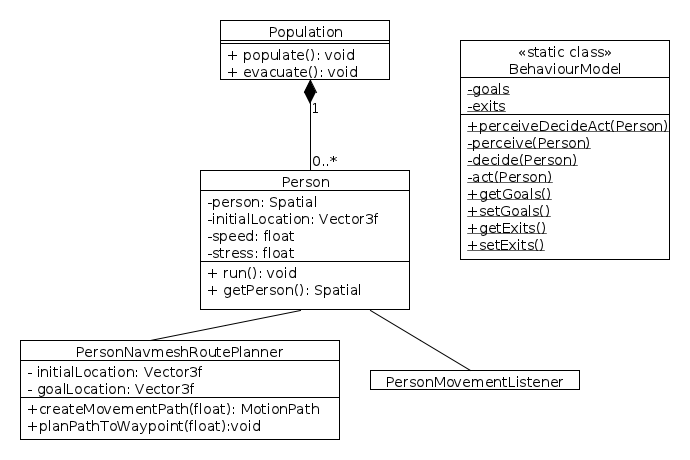
\includegraphics[scale = 0.5]{../UMLDiagrams/PopulationModel.png}
\caption{Population Package}
\label{fig:populationmodel}
\end{figure}


Figure \ref{fig:populationmodel} shows the relationship between the various classes responsible
for the realisation of autonomous agents and their behaviour within the simulator.
\\
The Population class represents the set of agents. A Population instance is ran as a separate thread of execution which
incrementally performs computations on the entire set of agents. It is also responsible
for the generation of the set of agents using the information provided in a set of PersonCategories (not shown) and the initiation
of agent evacuation.
\\
BehaviourModel is a static class designed to implement the Perceive, Decide, Act process (see Section \ref{Res:subsec:perceiveDecideAct}. For each step there is a corresponding 
private method which is called. The output from the perceive method, a list of goals visible to the agent, is passed to the decide method
which chooses a new target location for the agent to plan a path towards, and this location is passed to the act method which initiates the agents
movement towards its new goal.
\\
The seperation of these three stages is important to maximise the extensibility of the behavioural model. As mentioned, the decide method processes a set of
goals and, based on a set of rules and heuristics, chooses a new location for the agent. To change or extend the range of decisions an agent can make,
the programmer can simply add new rules to the decide method. In fact it is possible that multiple decision methods could be added where each implements
a different behavioural model. The only restriction is that the decide method must take a set of Goals (see below) as one of its inputs and must output a 3D point.
By calling the perceiveDecideAct method, an agent is taken through all three stages of the process and need have no knowledge of the decision algorithms used to select this new goal.
\\

An agent is primarily realised by the three classes: Person, PersonMovementListener and PersonNavmeshRoutePlanner. 
Each Person holds the attributes, including speed and stress (see Section \ref{Res:subsec:unifyingParameters}) which represent the characteristics of 
an evacuee. It also coordinates the visual representation of an agent and the movement of the agent towards its goal.
\\
In order to plan a route to a location, a Person must create a PersonNavmeshRoutePlanner instance. Its purpose is to act 
as if it were a `ghost' agent: it rapidly traverses the navmesh to establish a route. This route is then returned for the 
agent to move over. A fresh instance of PersonNavmeshRoutePlanner should be used every time a new route must be calculated and can be disposed
of once the route has been returned.
\section{Goals}
\label{Des:sec:goals}
\begin{figure}[here]
\centering
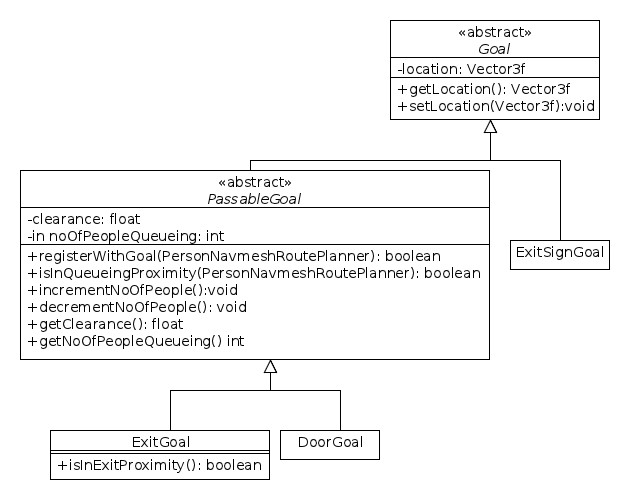
\includegraphics[scale=0.5]{../UMLDiagrams/GoalModel.png}
\caption{Hierarchy of goal package.}
\label{fig:goalhierarchy}
\end{figure}

A goal can be defined as anything in the environment which can steer an agent's direction. Figure \ref{fig:goalhierarchy} shows the inheritance hierarchy for goals in this simulation. At the top level we define a generic Goal, which simply has a location and does not direct agents explicitly.
\\
A PassableGoal is any goal through which an agent can move, such as a door or exit. These also have a clearance: a radius around its center which defines the maximum distance at which an agent can be considered to be queueing at that goal. This is vital for the computation of queueing behaviours. The number of people queueing at a PassableGoal is also stored and must be updated externally by agents as they approach or leave the goal.
Exits are represented by ExitGoals which are equipped with methods for recognising when an agent is close enough to exit the simulation.
\\
ExitSignGoal is an example of a non-passable goal which could direct agents to another goal. However non-passable goals are out of the scope of this project. ExitSignGoal is shown here purely to demonstrate that the existing framework could be extended to include such goals in future work.
\\
\\
\begin{figure}[here]
\centering
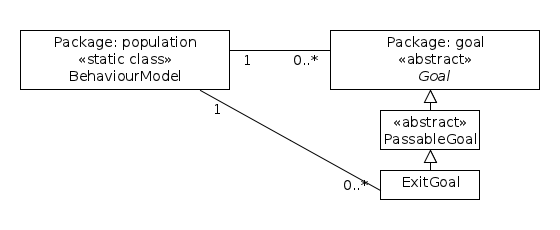
\includegraphics[scale=0.7]{../UMLDiagrams/BehaviourModelToGoalModel.png}
\caption{Relationship between BehaviourModel and Goals}
\label{fig:behaviourtogoalmodel}
\end{figure}

As Figure \ref{fig:behaviourtogoalmodel} shows, the static BehaviourModel instance holds a collection of all Goals in the simulation. For the purposes of calculating agent's paths out of the environment, a collection of all the ExitGoals is also kept separately, since it is anticipated that these will be used most frequently in calculations.\\

%\end{document}


%\documentclass{l3proj}
%\usepackage{graphicx}
%\usepackage{float}
%\usepackage{caption}
%\usepackage{subcaption}


%\begin{document}
%\title{Project Title}
%\author{Michael Kilian \\
%        Tony Lau \\
%        Dan Tomosoiu \\
%        Hector Grebbell \\
%        Peeranat Fupongsiripan}
%\date{13 March 2013}
%\maketitle



\section{Using the 3D Model}
\subsection{jMonkey Model Import}
Once the 3D model of the evacuation environment has been completed using Blender, it needs to be converted to a logical data structure (in this case, a Navigation Mesh) that can be used by the project for path-finding purposes. The first step of creating this structure is to convert the Blender file into a jMonkeyEngine (jME) compatible file. This process can be done automatically with the help of the jMonkey Integrated Development Environment: the file created in Blender is converted to a binary encoding of the mesh, which can be interpreted by jME. Once created, this file is permanently stored as a project asset and can be used whenever the user wishes to simulate an evacuation on that specific model.
The next step in creating the compatible data structure is to read the binary encoding of the environment and transform it into an initial jME mesh. This is a geometric mesh consisting of collections of three types of geometric primitives:
\begin{itemize}
  \item\textbf{Points}: Holds a vertex representing a single point in space
  \item\textbf{Lines}: Two vertices representing a line segment
  \item\textbf{Triangles}: Three vertices representing a solid triangle primitive
\end{itemize}
In this particular case, the jME mesh will hold the environment's geometric information using a list of 3D triangles, that were mapped from the imported model's surfaces.

\begin{figure}[H]
	\centering
	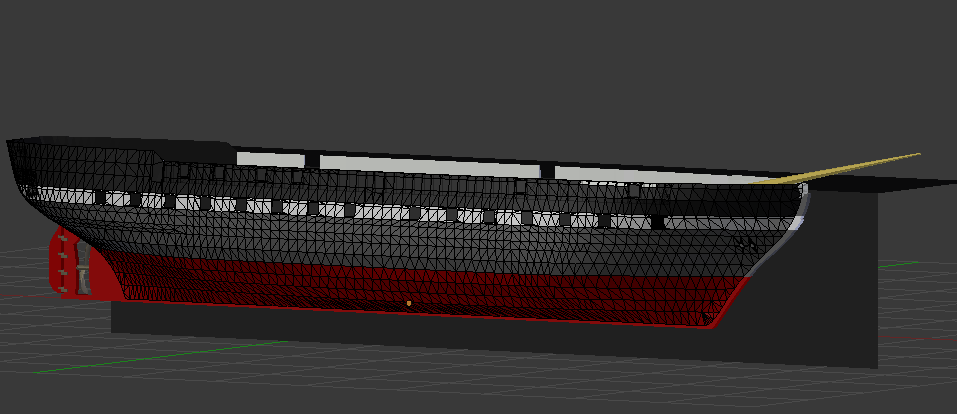
\includegraphics[width=1\textwidth]{../images/wireframe.png}
	\caption{View of the Blender model}
\end{figure}

\subsection {Choice of data structure}
In order to simulate a person's movement in the environment, we need a way to store and use information about its walkable surfaces.
A matrix-type structure, or a grid, is easy to visualise and implement. Surfaces are divided into tiny cells of the same size, each holding information about the type of surface it maps, and links to its neighbours. However this is costly in terms of memory consumption and processing power, as we will need a very large amount of cells for reasonably large environments.\\
A more efficient alternative are Navigation Meshes, as convex polygons are used to cover the walkable surface areas. This way, large open areas can be covered by a handful of polygons, greatly reducing the amount of memory needed. Since each individual polygon can still be considered a node, holding references to its neighbours, the whole structure can be used as a graph, which will later allow us to use efficient pathfinding algorithms, such as Dijkstra or A*.\\
Since 3D environment models contain information about more than just the walkable surfaces, a series of algorithms have to be used to extract and filter it into a navigation mesh.


\subsection{Conversion to a Navigation Mesh}
In order to allow agents to navigate over a mesh, a collection of the 3D surfaces (in this case, interconnected triangles) can be used. Any point interior to these triangles represents a valid location at which an agent can be positioned at any point in time. Furthermore, the agent can move from any point inside the triangle's surface to any other point inside the same surface.\\
Each of these triangles can have references (links) to zero to three other neighbouring triangles, one for each edge of the triangle. If a link exists between two triangle (i.e. they share a common edge), this means that an agent can traverse from one triangle to the other or vice-versa. As a result, a collection of such triangles, or cells, is a convenient structure on which to use graph path-finding algorithms: every cell can be interpreted as a graph node, and any link to other cells as a vertex between two nodes. This whole collection of interconnected triangles (cells), which can be abstracted as a graph, is called a Navigation Mesh (navmesh).\\
The Recast\cite{Recast} project is an open-source tool-set focused on the creation of navigation meshes from geometry meshes. The jMonkeyEngine's navmesh package, which is based on Recast, was used in order to convert the project's imported environment models into agent-navigable structures.\\
To create a navigation from an existing geometry mesh, a series of sequential processes is required. A summary of these processes and their parameters and results will be discussed next, based on the NMGen study \cite{NMGen}.
\begin{enumerate}
  \item\textbf{Voxelisation}: Create a solid height-field from the source geometry, made from a collection of voxels. A voxel (volumetric pixel) is a 3-dimensional, box-shaped unit used in representations of 3-dimensional images;


\begin{figure}[H]
	\centering
	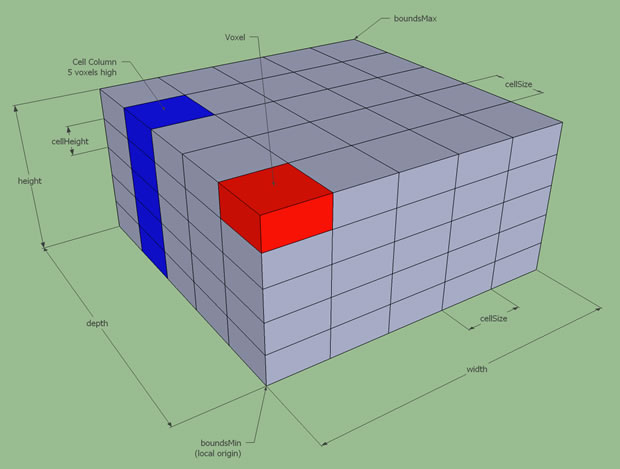
\includegraphics[width=1\textwidth]{../images/hf_03_voxelgrid.png}
	\caption{A voxel grid}
\end{figure}
  
  \item\textbf{Region Generation}: Detect the top surface area of the solid height-field and divide it up into regions of contiguous spans;
  
  
  \begin{figure}[H]
        \centering
        \begin{subfigure}[b]{0.48\textwidth}
                \centering
                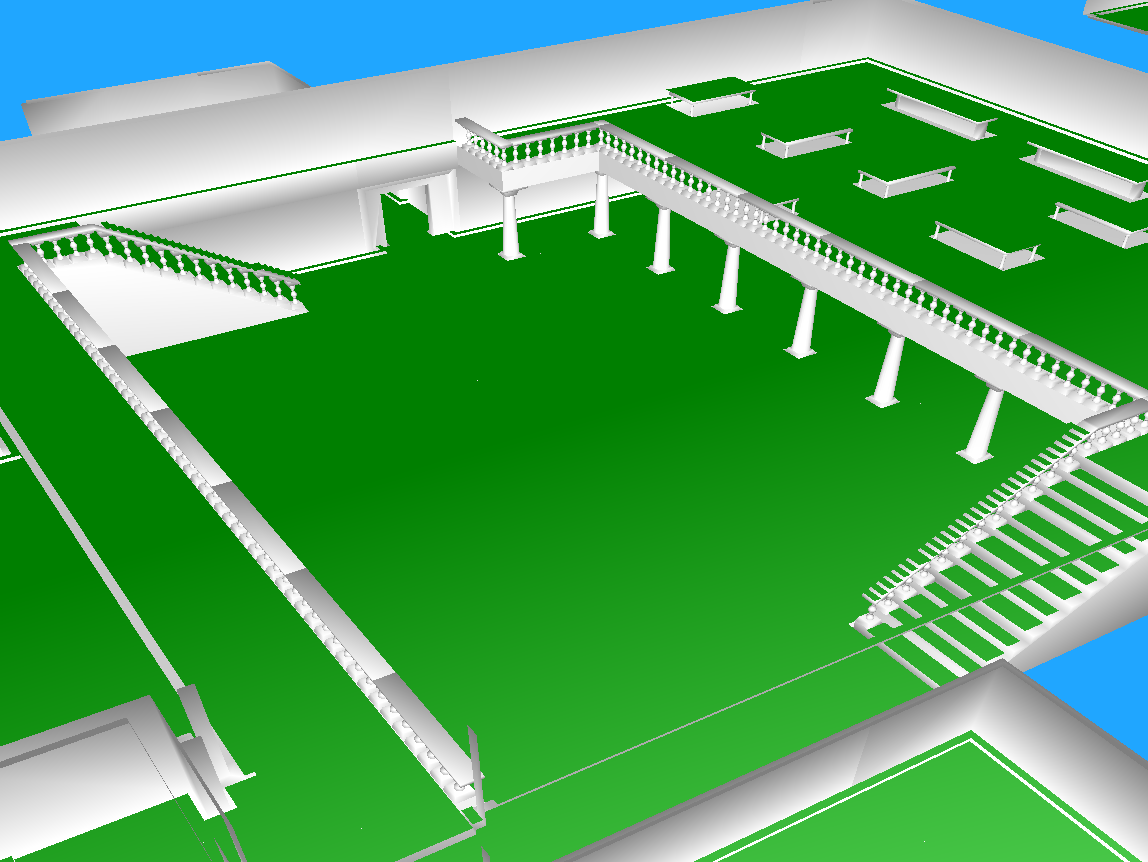
\includegraphics[width=\textwidth]{../images/region_generation.png}
                \caption{Overview of the model}
        \end{subfigure}
        \begin{subfigure}[b]{0.48\textwidth}
                \centering
                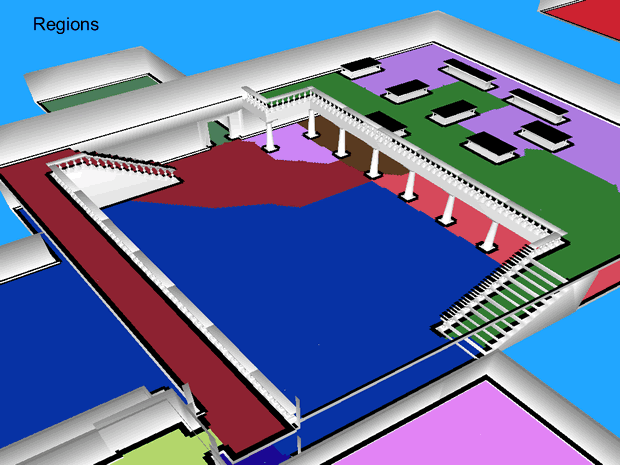
\includegraphics[width=\textwidth]{../images/stage_regions.png}
                \caption{Model split into regions}
        \end{subfigure}
        \caption{Region generation}
	\end{figure}        

  \item\textbf{Contour Generation}: Detect the contours of the regions and form them into simple polygons;

  
  \item\textbf{Convex Polygon Generation}:  Sub-divide the contours into convex polygons;
  
  \begin{figure}[H]
        \centering
        \begin{subfigure}[b]{0.48\textwidth}
                \centering
                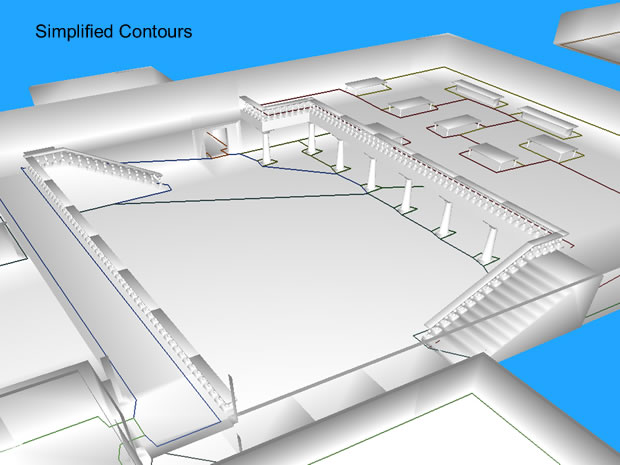
\includegraphics[width=\textwidth]{../images/cont_11_simplified_full.png}
                \caption{Contour generation}
        \end{subfigure}
        \begin{subfigure}[b]{0.48\textwidth}
                \centering
                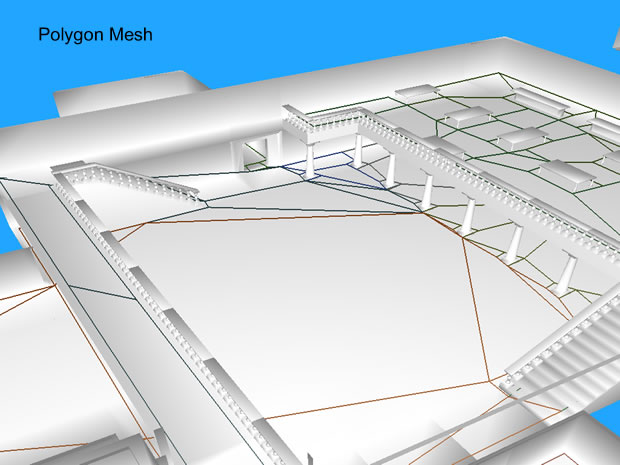
\includegraphics[width=\textwidth]{../images/stage_polygon_mesh.png}
                \caption{Convex polygon division}
        \end{subfigure}
        \caption{Region generation}
	\end{figure}   
  
  
  
  
  
  \item\textbf{Detailed Mesh Generation}: Triangulate the polygon mesh and add height detail.
  
  \begin{figure}[H]
	\centering
	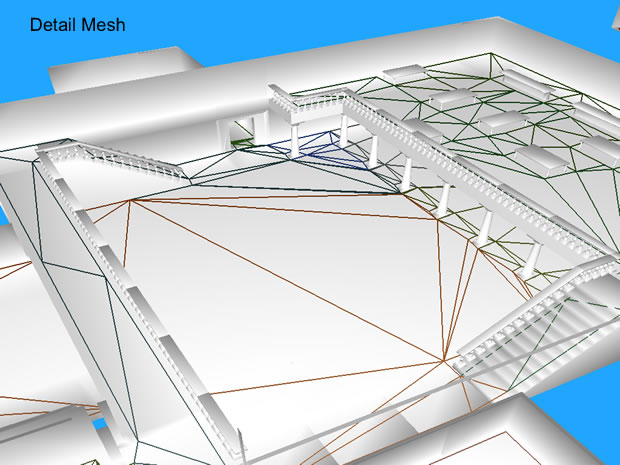
\includegraphics[width=1\textwidth]{../images/stage_detail_mesh.png}
	\caption{Detailed mesh}
\end{figure}  
  
\end{enumerate}


In order to obtain a well-formed mesh, several parameters are required to be passed to the generator (note: where parameters are dependent on variables like agent surface area or agent height, the corresponding values should be calculated in relation to the scale of the imported model):
\begin{itemize}
  \item\textbf{Cell size}: Represents the width and depth of the voxel units which will fill the source geometry. This parameter will influence the accuracy of the generated navigation mesh in relation to the supplied geometry mesh. Lower values closely make the result closely match the source geometry but with a proportional increase in computation time and space costs. In order for the navmesh to be well-formed, this parameter needs to be at least several times smaller than the size of an agent's surface area.
  
  \item\textbf{Cell height}: Represents the height of the voxels used to create the solid height-field. Like the width and depth, the height of the voxel influences the level of accuracy of the navmesh. A well-formed navmesh requires this parameter to be at least several times smaller than the height of an agent's maximum step (step-height).
  
\begin{figure}[H]
	\centering
	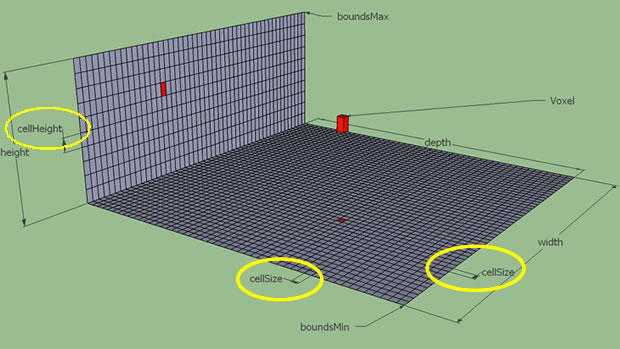
\includegraphics[width=1\textwidth]{../images/cell_size_height.png}
	\caption{Cell size and height}
\end{figure}   

  
  \item\textbf{Minimum traversable height}: Represents the minimum distance from the floor to the ceiling that will still allow an agent to pass through. Should be at least the size of maximum agent height. Should also be at least two times the height of a voxel (cell height).
  
  \begin{figure}[H]
	\centering
	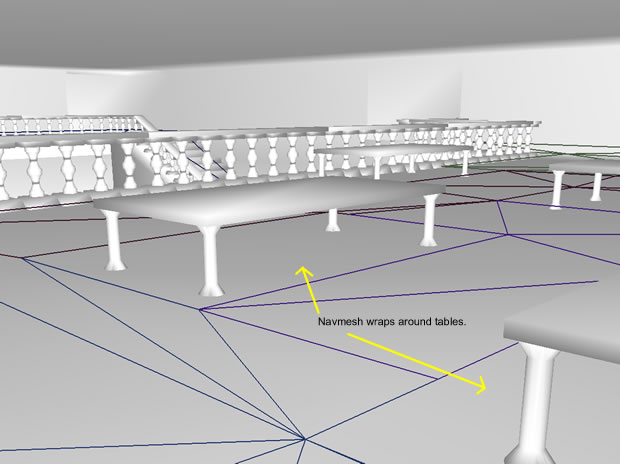
\includegraphics[width=1\textwidth]{../images/main_walkheight_norm.png}
	\caption{When minimum traversable height set correctly, the mesh does not flow under the tables}
\end{figure}   
  
  \item\textbf{Maximum traversable step}:  Represents the maximum height of a ledge that can be climbed by an agent. Should be at least twice the height of a voxel.
  
\begin{figure}[H]
	\centering
	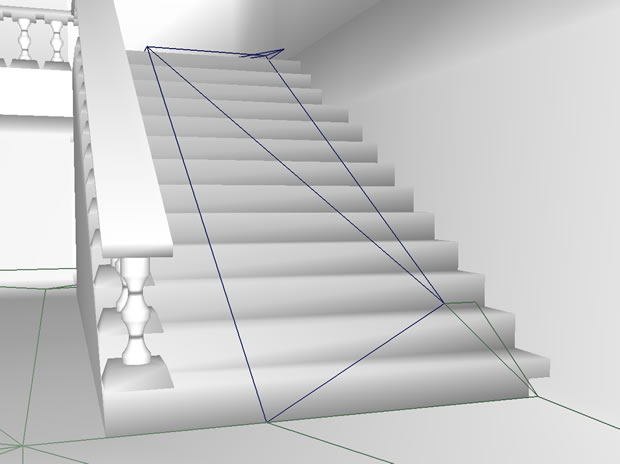
\includegraphics[width=1\textwidth]{../images/max_trav_step.png}
	\caption{Setting a correct value for the maximum traversable step, elements such as stairs can be detected and made walkable}
\end{figure} 
  
  \item\textbf{Maximum traversable slope}: Represents the maximum slope of a ramp that is still deemed traversable. Any ramps with a higher slope will be considered unwalkable and will be considered an obstacle by the navmesh.
  
  \item\textbf{Border size of traversable area}: Represents the distance from the walls to the actual walkable area. For a well-formed navmesh, this should be at least the same size as an agent's surface area.
  
	\begin{figure}[H]
	\centering
	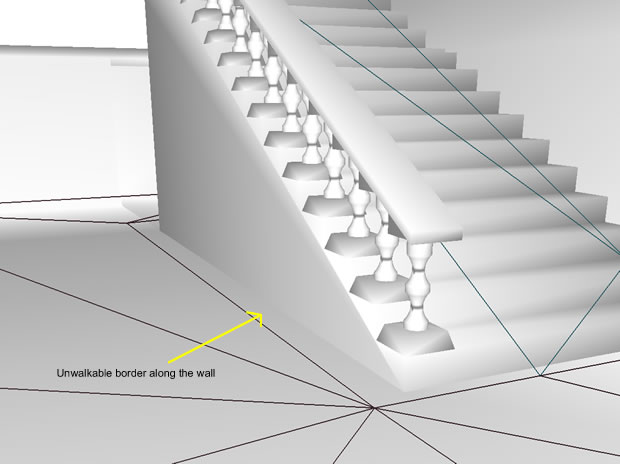
\includegraphics[width=1\textwidth]{../images/border_trav_size.png}
	\caption{The walkable surface will be limited to at least the size of the border. Setting the border size to at least the size of an agent's surface area enables the agent to be positioned on any point of the mesh, without worrying of contact with the walls}
\end{figure} 

  
  \item\textbf{Smoothing threshold}: The amount of smoothing (larger region size, fewer thin triangles) to be performed when generating the distance field
  
%  	\begin{figure}[H]
%	\centering
%	\includegraphics[width=1\textwidth]{smoothing_0.png}
%	\caption{Smoothing disabled}
%\end{figure}
%
% 	\begin{figure}[H]
%	\centering
%	\includegraphics[width=1\textwidth]{smoothing_1.png}
%	\caption{Smoothing enabled}
%\end{figure}  


\begin{figure}[H]
        \centering
        \begin{subfigure}[b]{0.48\textwidth}
                \centering
                \includegraphics[width=\textwidth]{../images/smoothing_0.png}
                \caption{Smoothing disabled}
        \end{subfigure}
        \begin{subfigure}[b]{0.48\textwidth}
                \centering
                \includegraphics[width=\textwidth]{../images/smoothing_1.png}
                \caption{Smoothing enabled}
        \end{subfigure}
        \caption{Smoothing threshold}
	\end{figure}        

  
  \item\textbf{Minimum size of unconnected region}: Represents the surface, in voxels, of regions that should not be added to the navmesh if they are unconnected to other regions (i.e. islands).
  
  

\begin{figure}[H]
        \centering
        \begin{subfigure}[b]{0.49\textwidth}
                \centering
                \includegraphics[width=\textwidth]{../images/min_unconn_region_0.png}
                \caption{A correct value for the minimum unconnected region size does not create a mesh surface for the table tops}
        \end{subfigure}
        \begin{subfigure}[b]{0.49\textwidth}
                \centering
                \includegraphics[width=\textwidth]{../images/min_unconn_region_1.png}
                \caption{Setting the value of the minimum unconnected region size too low, the table tops are interpreted as walkable surfaces}
        \end{subfigure}
        \caption{Minimum unconnected region size}
	\end{figure}        


  
%  \begin{figure}[H]
%	\centering
%	\includegraphics[width=1\textwidth]{min_unconn_region_0.png}
%	\caption{A correct value for the minimum unconnected region size does not create a mesh surface for the table tops}
%\end{figure}
%  
%  \begin{figure}[H]
%	\centering
%	\includegraphics[width=1\textwidth]{min_unconn_region_1.png}
%	\caption{Setting the value of the minimum unconnected region size too low, the table tops are interpreted as walkable surfaces}
%\end{figure}
  
  \item\textbf{Merge region size}: Represents the minimum number of voxels a region should have in order to not try and merge it with other adjacent regions. This influences the number of long thin regions.
  
  
  \begin{figure}[H]
        \centering
        \begin{subfigure}[b]{0.49\textwidth}
                \centering
                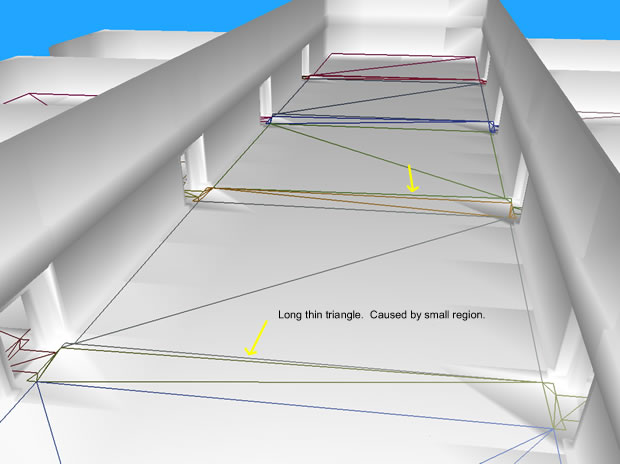
\includegraphics[width=\textwidth]{../images/merge_region_0.png}
                \caption{With merge region size set too low, the surfaces can be covered by a large number of long thin triangles}
        \end{subfigure}
        \begin{subfigure}[b]{0.49\textwidth}
                \centering
                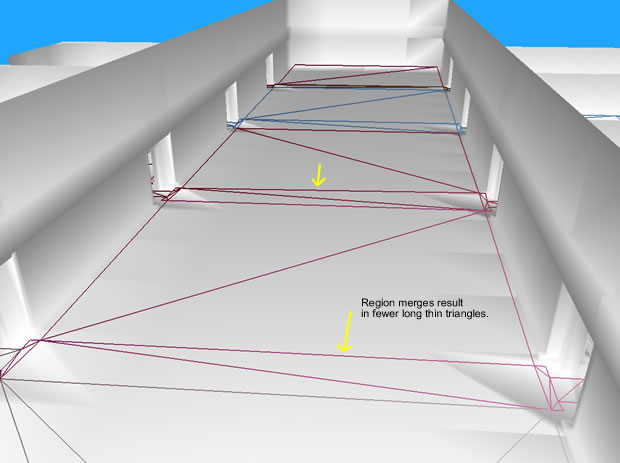
\includegraphics[width=\textwidth]{../images/merge_region_1.png}
                \caption{Setting the merge region size to a large enough value, some of the thin triangles are merged together with adjacent triangles (where possible)}
        \end{subfigure}
        \caption{Merge region size}
	\end{figure}  
  
  \item\textbf{Maximum edge length}: Represents the maximum length of a triangle's edge. If a triangle has a greater length, it will be split into several legal triangles, by adding more vertices on the border edges.
  
  \begin{figure}[H]
	\centering
	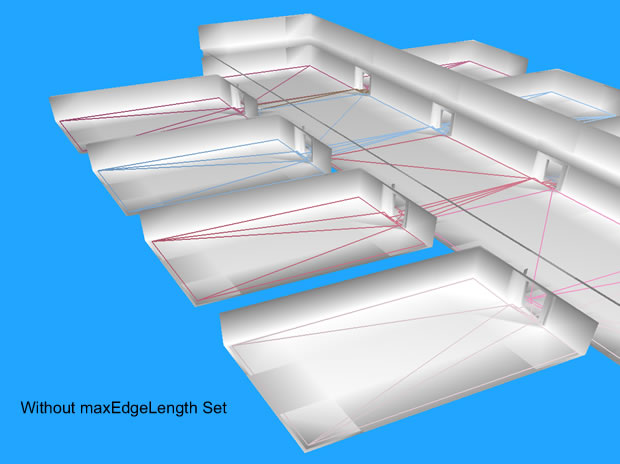
\includegraphics[width=1\textwidth]{../images/max_edge_0.png}
	\caption{With the maximum edge length setting disabled, very long triangles can be generated}
\end{figure}

  \begin{figure}[H]
	\centering
	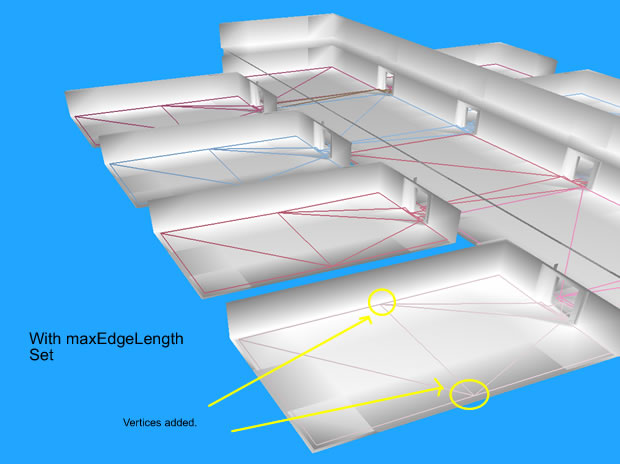
\includegraphics[width=1\textwidth]{../images/max_edge_1.png}
	\caption{With the maximum edge length setting enabled, more vertices are added along the edge of the initial long triangles}
\end{figure}
  
  \item\textbf{Edge maximum deviation}: Influences the accuracy of the edges following the source geometry. The lower the value, the higher the accuracy, but at increased triangle count and processing cost.
  
  \begin{figure}[H]
	\centering
	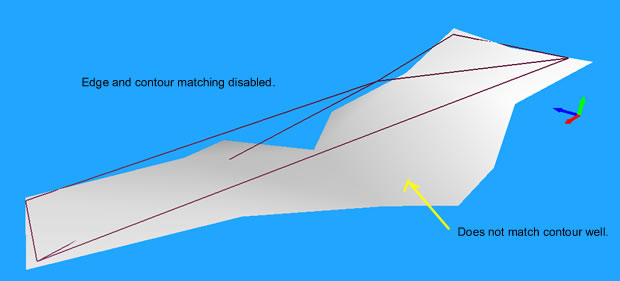
\includegraphics[width=1\textwidth]{../images/edge_dev_0.png}
	\caption{Edge maximum deviation disabled}
\end{figure}
\begin{figure}[H]
	\centering
	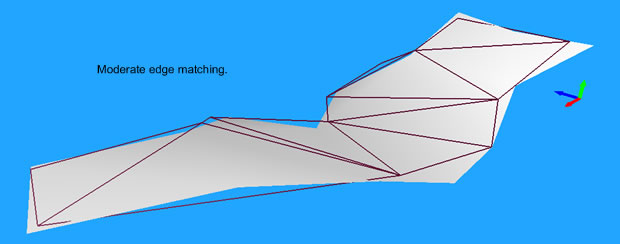
\includegraphics[width=1\textwidth]{../images/edge_dev_1.png}
	\caption{Moderate edge matching}
\end{figure}
\begin{figure}[H]
	\centering
	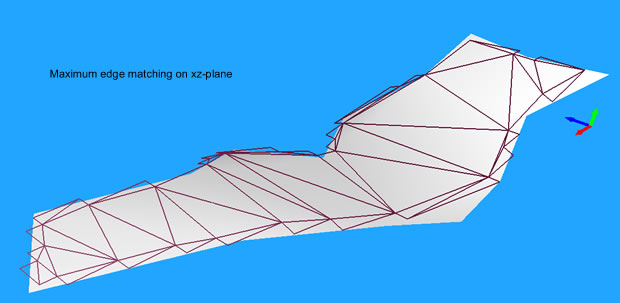
\includegraphics[width=1\textwidth]{../images/edge_dev_2.png}
	\caption{Higher fidelity edge matching}
\end{figure}
  
  
  \item\textbf{Max vertex per polygon}: If set to higher than 3, increases the cost of the computation but can result in better formed regions. However, for the current project, a value of 3 should be used, since the algorithms designed for path-finding only support 3-sided cells.
\end{itemize}
	

The problem that arises with such a high number of variables is the fact that end-users will not be able to import new models from different evacuation environments without a significant overhead. If wrong parameters are used for the mesh generation, the set of algorithms used might generate badly formed meshes, which do not map the source environment closely enough or even fail all-together.
Still, with proper scaling of the model, either in Blender stage or after importing the geometrical mesh, importing models of different magnitudes can be achieved.\\

Since the space available for this report is limited, navigation mesh generation was presented only succinctly. For more in-depth information about each of the steps taken and how the previously discussed parameters influence the resulted mesh, the reader can refer to the NMGen Project documentation \cite{NMGen}.
\section{Navigation}

\subsection{Logical structure}

\begin{figure}[H]
	\centering
	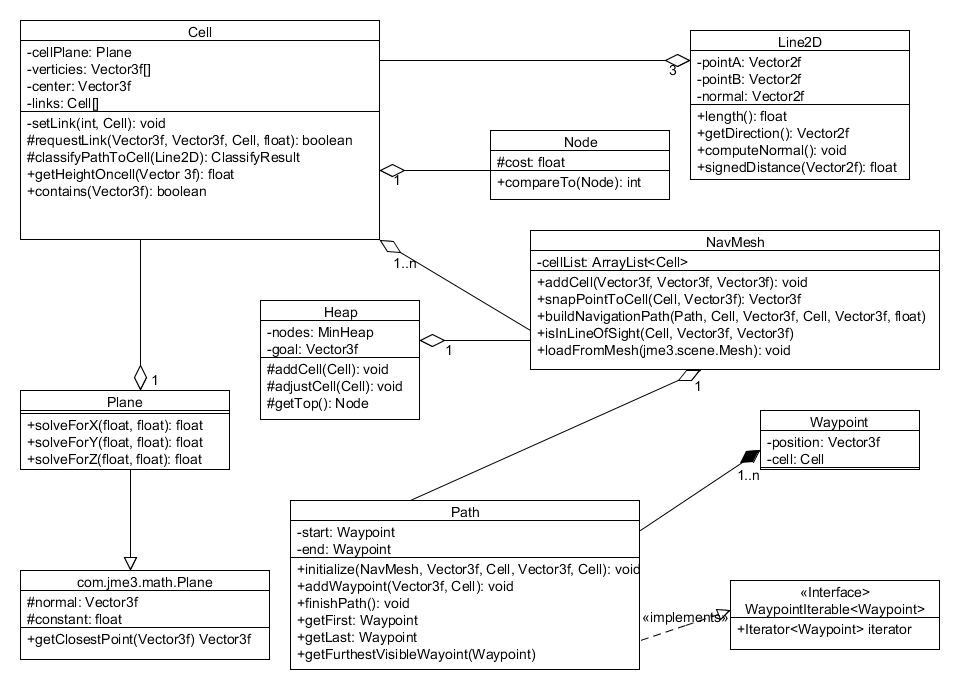
\includegraphics[width=1\textwidth]{../images/navmesh.png}
	\caption{Navmesh Package}
	\label{fig:navmesh_package}
\end{figure}

Figure \ref{fig:navmesh_package} shows the relationship between the various classes responsible for path generation. The NavMesh class contains a list of Cells, each being a triangle representing a piece of the surface mapped by the mesh. Each cell has references to its three vertices (of Vector3f type), its three edges (of Line2D type) and its corresponding neighbours, or links (of type Cell) - three or less, depending on the number of neighbours. Each cell also has a corresponding plane reference, used to help with computing 3D calculations.
The NavMesh initialisation is made by calling the loadFromMesh method, with the mesh resulted from the previous generation step as a parameter. As a result, the cell list will be populated with the relevant data. \\
Upon creation, each agent object representing a person will be assigned a new Path. By initialising the path with the relevant NavMesh reference, each agent can then independently use the reference to call the NavMesh's buildNavigationPath method. While calling this method, the Path in which to write the result is passed as a parameter, along with the start-point vector and end-point vector, the respective cells in which each vector reside, and a floating point number representing the size of the increments in which to place waypoints. More details about the way the path is calculated will be provided in the next section~\ref{pathfinding}. \\
Once the buildNavigationPath has returned control to its caller, the Path passed as a parameter will contain a list of Waypoints - a tuple of intermediary vectors, in increments of the floating point number provided, along with the cells in which each vector reside. Since Path implements the Iterable interface, the agent owning it can simply iterate over the waypoints contained and move along them sequentially.

\subsection{Pathfinding}
\label{pathfinding}

The buildNavigationPath method from the NavMesh class is in charge of the actual pathfinding routine. Since the navigable surface of the environment is mapped into cells which link to their neighbouring cells, this data structure can be regarded as a non-oriented graph. Therefore, graph pathfinding algorithms like Dijkstra\cite{Dijkstra} or A*\cite{Astar} can be used.  While the number of agents required for the initial environment is small (200), A* would be a more scalable option, being faster than Dijkstra thanks to heuristics which attempt to preempt the optimal path.\\
The pathfinding method used in buildNavigationPath is using A*: a priority queue structure (MinHeap) is used to store intermediary paths from the source to destination, sorted by their lowest expected cost. The heuristic function used in the A* implementation is the euclidean distance from the center of the current cell to the goal. This distance is added to the total cost of the route up to the current location, and based on these data for each of a current cell's neighbours, decisions are made to consider the cells for further paths or ignore them.\\
Once the calling agent receives control back from the method, the Path passed as a parameter will hold a valid route from the agent's position to its destination, and can be used for scheduling movement.

%\bibliographystyle{plain}
%\bibliography{teamL_dissertation_2013}
%\end{document}
 %not complete

%==============================================================================
\chapter{Implementation}
\label{implementation}

%\documentclass{article}
%\usepackage{algorithm2e}
%\begin{document}
\section{Route Planning}
\label{Imp:sec:routePlanning}
Planning an agent's route from its current point to a given point is acheived by a collaboration between a Person and PersonNavmeshRoutePlanner instance. Routes are stored using the jMonkeyEngine class MotionPath. This contains a set of waypoints and methods to animate the agent's movement between these waypoints. The maximum distance between each waypoint is roughly constant and can be set as a parameter to the following procedure (it is not constant when the agent must turn at a point closer to its current position that the maximum distance between points). The distance used is an important decision in the implementation. If it is too large the accuracy of the animation tends to degrade. If it is too low then a large number of waypoints will be stored needlessly. After extensive experimentation 0.5 was found to be an acceptable value for the maximum distance between waypoints. In practice this provided a balance between quality and efficiency.\\
A route is calculated in two stages:
\begin{enumerate}
\item{A path is calculated on the navigation mesh using a modified A* algorithm to traverse the mesh like a graph. This returns a small set of points. These points illustrate the lines of motion an agent must take to reach their goal. This is performed in the constructor for a PersonNavmeshRoutePlanner.}
\item{Using these points as guidance, the path is `fleshed out' by moving along the path and placing MotionPath waypoints no further apart than the defined maximum
distance. This terminates with a waypoint being placed on the goal location the agent must reach.}
\end{enumerate}
Note that a fresh PersonNavmeshRoutePlanner instance must be instantiated to calculate a route. The relationship between the Person and PersonNavmeshRoutePlanner instances is expressed in \ref{fig:RoutePlanSequence}.

\begin{figure}
\label{fig:RoutePlanSequence}
\centering
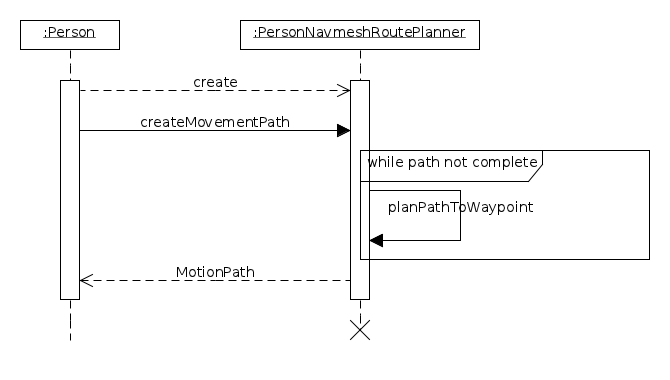
\includegraphics[scale=0.5]{../UMLDiagrams/RoutePlanningSequence.png}
\caption{Generation of an agent route as a MotionPath}
\end{figure}


\section{Implementing the Perceive, Decide, Act Process}
\label{Imp:sec:perceiveDecideAct}
Here we discuss the techniques and algorithms used to realise the Perceive, Decide, Act process previously discussed in Section \ref{Res:subsec:perceiveDecideAct}.

%%%%%%%%%%%%%%%%%%%%%%%%%Perception Implementation
\subsection{Perception}
\label{Imp:subsec:perception}
Agent perception is achieved using the following simple algorithm:

\begin{algorithm}[H] %%%%%%%Agent Perception Algorithms
 \SetAlgoLined
 \SetKwInOut{Input}{input}
 \SetKwInOut{Output}{output}
 \Input{The set of goals in the environment: \emph{goals}}
 \Output{A set of goals visible to the user at the given instant in time: \emph{visibleGoals}}
 \BlankLine
 \For{each goal g in goals}{
  \If{g is in line of sight of agent}{
    add g to visibleGoals\;
  }
  }
  \caption{Agent Perception Algorithm}
\end{algorithm}

%%%%%%%%%%%%%%%%%%%%%%%%%%%%%Decision Implementation
\subsection{Decision}
\label{Imp:subsec:decision}
In the Research Chapter [Reference] the three classes of human behaviour considered in the scope of this project were defined. In practice, only herding behaviour implemented as part of the Decide step; queueing and competetive behaviour must be handled asynchronously using collision avoidance techniques. Unfortunately collison avoidance was not implemented in the final system due to various problems discussed in Section \ref{Problems:subsec:problemsecountered}. Future solutions to implement collision avoidance are discussed in Section \ref{Problems:subsubsec:ORCA}.
To decide on a new action, an agent must select one of the visible goals that were found in the Perceive step (if any). Otherwise it must continue on its current path. The decision making process is realised using an extendable algorithm, which sequentially considers sets of different classes of goal according to their priority. Exits have the highest priority.\\

The final algorithm only makes decisions regarding exits, due to various issues which emerged during development (see Section \ref{Problems:subsec:problemsecountered}). However it is easy to extend this process to include other goal types by adding further conditionals following the pattern laid out below.\\

%%%%%%%%%%%%%%%%%%%%%%%%%%%Decide Algorithm
\begin{algorithm}[H]
 \SetAlgoLined
 \SetKwInOut{Input}{input}
 \SetKwInOut{Output}{output}
 \Input{Person person, ExitGoal[ ] exits /*add further exit types here as arrays */}
 \Output{Target Goal for agent to move toward}
 \eIf{no of exits $>$ 0}{
   ExitGoal \emph{currentExit} = $exits[0]$\;
   \eIf{person is stressed}{
     \For{each exit \emph{e} in exits}{
       \If{number of people queuing at e $>$ no. of people queueing at targetExit}{
	targetExit = e\;
	}
      }
    return targetExit\;
    }{ %%%%%%%%%%%inner else
     Vector3f position = person.location\;
     \For{each exit e in exits}{
       \If{distance to e $<$ distance to targetExit}{
	targetExit = e\;
	}
      }
      return targetExit\;
     }
}{ %%%%%%%%outer else
  return null;
}
\end{algorithm}

\subsection{Act}
\label{Imp:subsec:act}
This step's representation in the BehaviouralModel class is trivial since the Decide step already returns a target goal. It is left in as a place for performing any calculations which should be performed before returning the target goal to the agent.\\
Upon receiving a new target goal, an agent should perform the following:
\begin{itemize}
\item{Use a PersonNavmeshRoutePlanner to calculate a route to this goal}
\item{Set the returned MotionPath as the current MotionPath for the agent}
\item{Begin moving down this path}
\end{itemize}




%\end{document}
     
     
 

    


%% LyX 2.0.3 created this file.  For more info, see http://www.lyx.org/.
%% Do not edit unless you really know what you are doing.
%\documentclass[english]{article}
%\usepackage[T1]{fontenc}
%\usepackage[latin9]{inputenc}
%\usepackage{graphicx}
%\usepackage{babel}
%\begin{document}

\section{GUI Design and Implementation}
\label{guidesign}

The target userbase for the evacuator does not guarantee a good degree
of computer-literacy. Hence a clear and easy to use GUI was required.


\subsection{Initial Design}

Based from initial system requirements a wireframe for the GUI could
be generated. To keep the user experience simple it was decided to
keep all the basic functionality within the main window. This allows
unfamiliar users to gain from the software without being overwhelmed
by endless options. For advanced configuration there was to be a detailed
configuration panel allowing advanced users to set the majority of
variables as they saw fit.

The wireframe below was drawn up to support these concepts. By sticking
to conventions it gives a familiar feel to most who have used a typical
windows based system within the last decade.\\

\begin{figure}
\centering
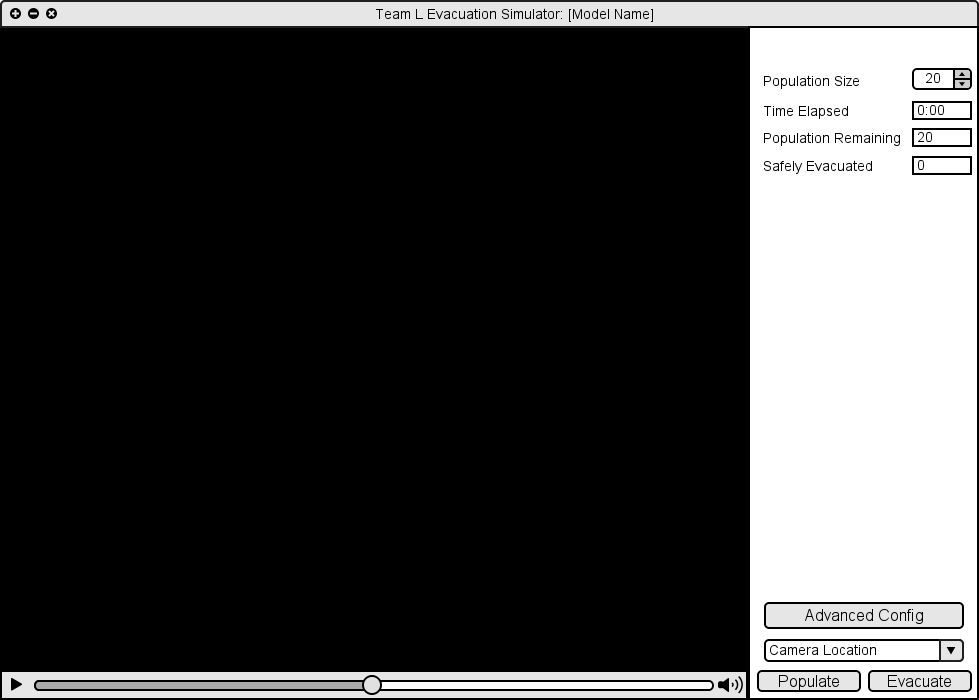
\includegraphics[width=10cm]{../images/GUIv1WF}
\caption{First attempt at wireframing GUI\label{ref:initialGUI}}
\end{figure}

%\caption{Sample configuration\label{fig:sampleconfig}}

\subsection{GUI Implementation and Revision}

It was decided since the project was to be built in Java and several
members had knowledge of the library to use Swing for implementation
of the GUI. The toolkit was more than capable of our needs and any
advantages of alternatives seemed unlikely to counterbalance the time
required to learn a new environment. SWT was briefly considered since
the interface created generally allows a closer to native feel and
higher performance \cite{SWT}.
This however would come at a cost of portability as well as the time
consideration mentioned above.

The initial GUI implementation (\ref{ref:initialGUI}) was a quick and crude attempt towards the initial
wireframe. Its purpose was more towards checking how well the JMonkey
canvas could be displayed within the Swing layout than producing a
suitable end product.\\

\begin{figure}
\centering
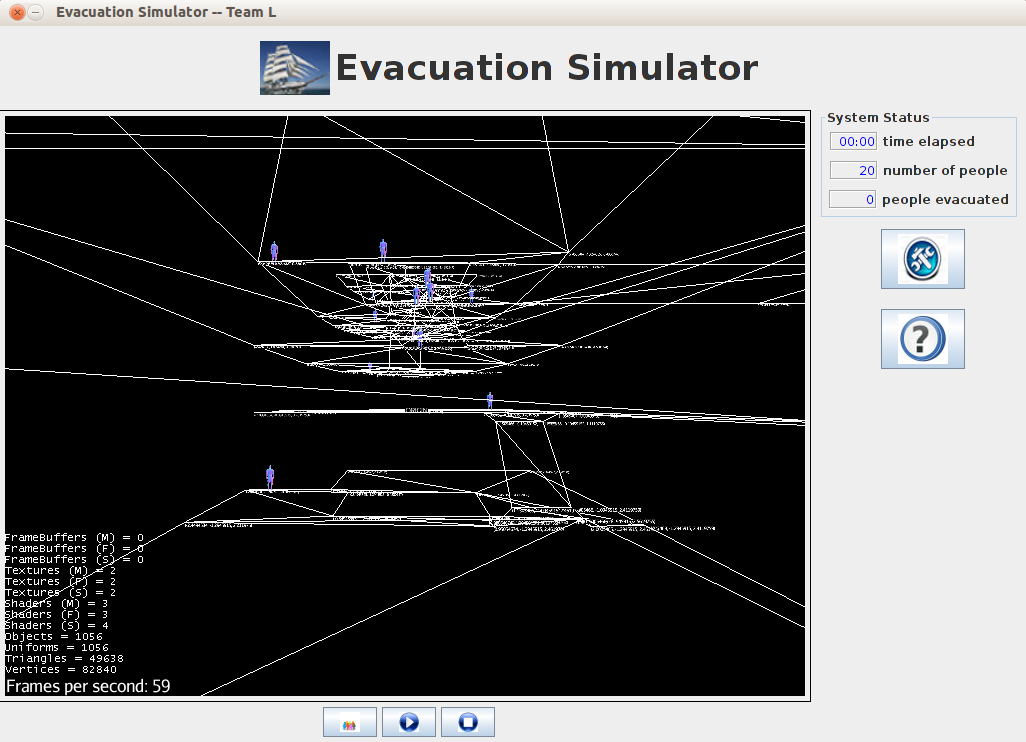
\includegraphics[width=10cm]{../images/GUIv1}
\caption{First refinement of GUI}
\end{figure}

Whilst not particurly attractive a suitable platform for basic testing
was then available.

At this point it became apparent that the back end would not easily
allow for the evacuation to be ``scrolled through'' in the way we
had initially anticipated. The play bar at the bottom of the screen
was removed from designs. this led to the control buttons being moved
to the panel on the right. After speaking to some less computer-literate
users it was further decided to use a traditional menu-bar. Some also
found the navmesh didn't give an immediate understanding of what
the model represented so toggles were added to allow a physical representation
of the ship to be shown.

These changes manifested themselves as can be seen in \ref{secondRefinementGUI}. Due to more
time being spent on this iteration it gives a much more complete feel
and is considerably closed to the initial wireframe.\\

\begin{figure}
\centering
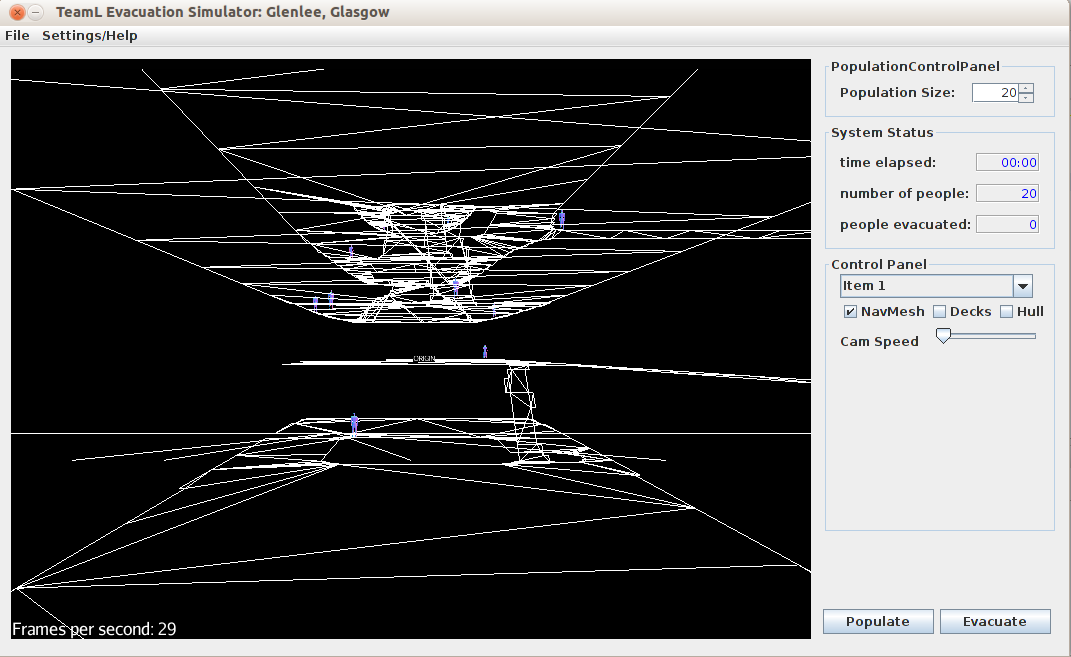
\includegraphics[width=10cm]{../images/GUIv2}
\caption{Second refinement to GUI\label{secondRefinementGUI}}
\end{figure}

Further talks with users suggested that for those not used to computer-games
the keyboard based camera controls were not immediately understandable.
To fix this a control panel was added. Due to the way functionality was implemented
a route button was added for testing purposes. It was then decided
this would be of use to users so was left in. Finally, to allow a
more native feel the theming was set to inherit from the system the
code was run from. A new wireframe (\ref{thirdRefinementGUI}) was drawn up  to
show this.\\

\begin{figure}
\centering
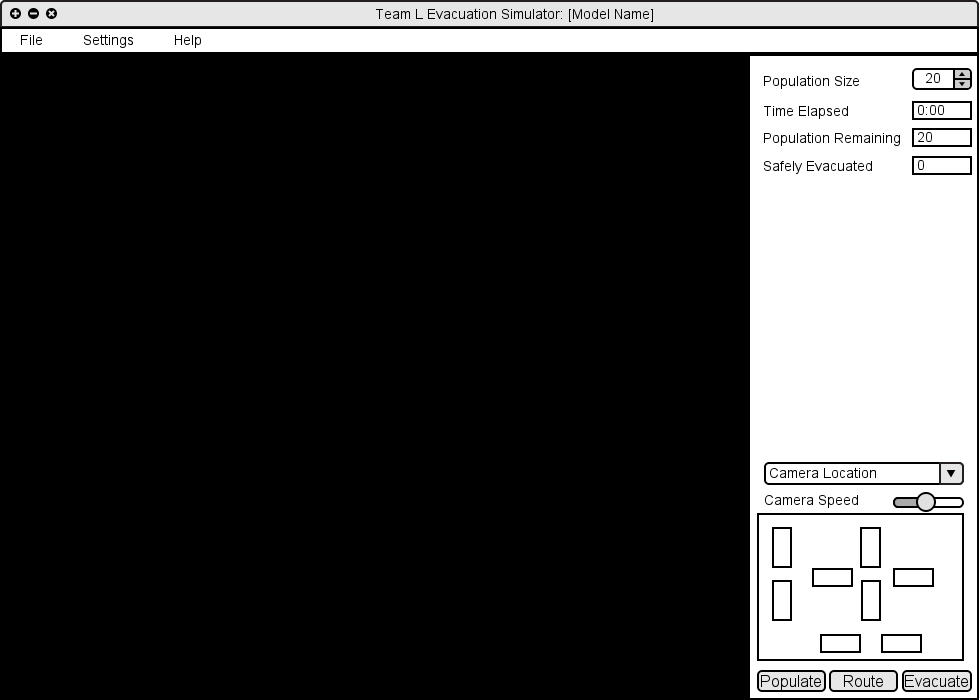
\includegraphics[width=10cm]{../images/GUIv2WF}
\caption{Third refinement to GUI\label{thirdRefinementGUI}}
\end{figure}

\subsection{Final GUI}

The wireframe in \ref{finalGUI1} was implmented to give our final GUI. It gives
a polished finish and meets original aims well and takes into consideration
user feedback. 

Initial work was done using the Netbeans GUI builder. This allowed
the layout we required to be built quickly, but not the functionality.
To achieve this some work was needed on the raw swing code.

The final interface is shown in \ref{finalGUI2}, both in Linux and Windows.\\

\begin{figure}
\centering
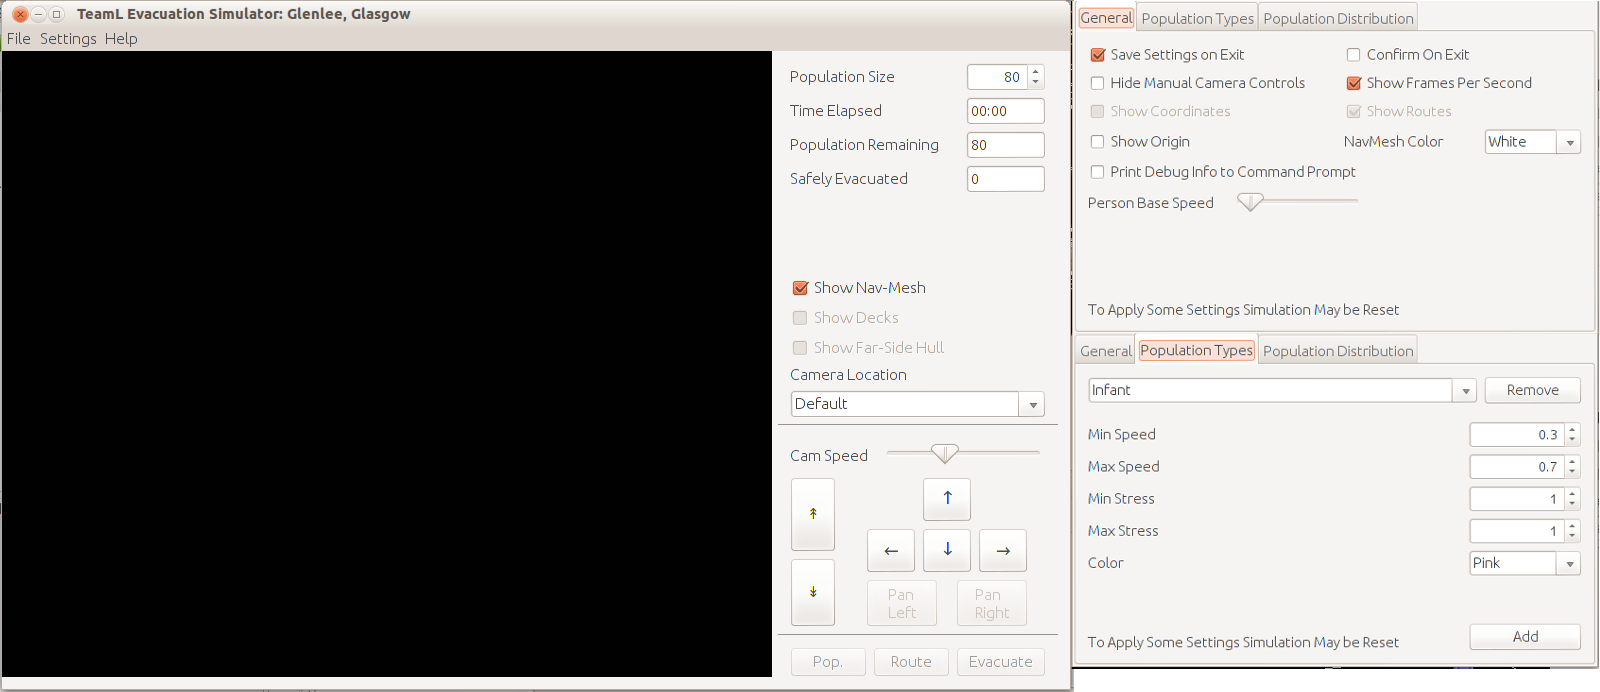
\includegraphics[width=18cm]{../images/GUIv3FULL}
\caption{Final GUI wireframe\label{finalGUI1}}
\end{figure}

\begin{figure}
\centering
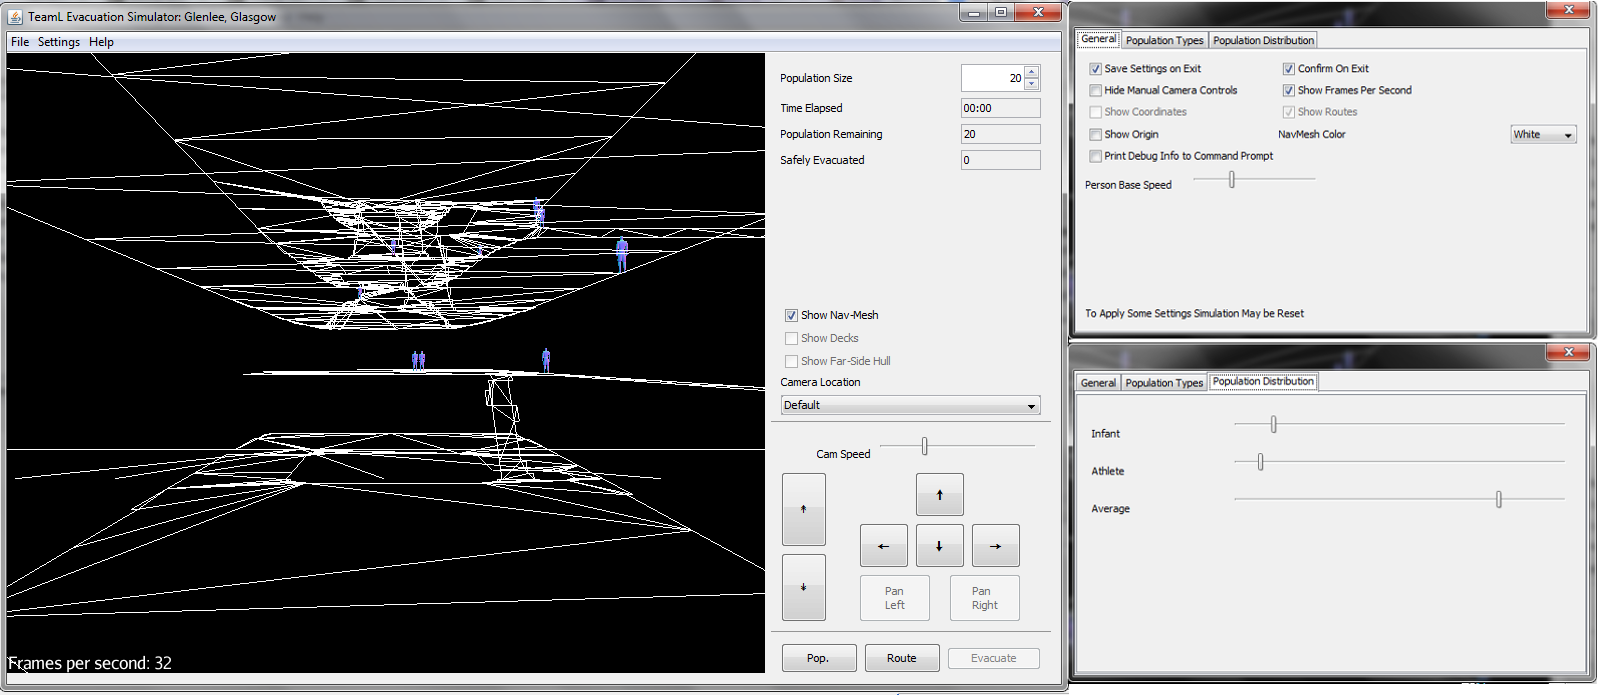
\includegraphics[width=18cm]{../images/GUIv3FULLWIN}
\caption{Final GUI in Swing\label{finalGUI2}}
\end{figure}


%\end{document}
 %not complete

%==============================================================================
\chapter{Evaluation}
\label{evaluation}

% This example An LaTeX document showing how to use the l3proj class to
% write your report. Use pdflatex and bibtex to process the file, creating 
% a PDF file as output (there is no need to use dvips when using pdflatex).

% Modified 

%\documentclass{article}
%\begin{document}
%\title{User Interface Evaluation}
%\author{Tony Lau}
%\maketitle
%==============================================================================
\section{User Interface Evaluation Methods}
\label{evalmethods}

The simulator will be evaluated through a series of user tests with different participants. The goals of the user interface evaluation are to assess the effect of the interface on the user and to identify specific problems which should be rectified. The simulator will be first tested with the fire warden of The Tall Ship who is the primary user of the system. Secondly, feedback on usability of the system will be gathered from usability testing with the subjects being students at the University of Glasgow.

Two evaluation methods, namely Heuristic Evaluation and Usability Experiments, will be used to determine whether the requirements specified in section \ref{requirements} have been met and also to determine the overall usability of the system.

\subsection{Heuristic Evaluation}
Heuristic evaluation is a usability inspection method pioneered by Jakob Nielsen and Rolf Molich which helps to identify problems with a user interface by judging the interface's compliance to recognized usability principles -- heuristics\cite{heuristics}.

The heuristics made use of in this part of the evaluation are Nielsen's Heuristics, developed by Jakob Nielsen and Rolf Molich in 1990\cite{tenheuristics}. Nielsen refined the original set of heuristics in 1994\cite{tenheuristics}. Below is list of the heuristics and a description of each one:
\\
\textbf{1. Visibility of system status:}
The system should always keep users informed about what is going on, through appropriate feedback within reasonable time.
\\
\textbf{2. Match between system and the real world:}
The system should speak the user's language, with words, phrases and concepts familiar to the user, rather than system-oriented terms. Follow real-world conventions, making information appear in a natural and logical order.
\\
\textbf{3. User control and freedom:}
Users often choose system functions by mistake and will need a clearly marked "emergency exit" to leave the unwanted state without having to go through an extended dialogue. Support undo and redo.
\\
\textbf{4. Consistency and standards:}
Users should not have to wonder whether different words, situations, or actions mean the same thing. Follow platform conventions.
\\
\textbf{5. Error prevention:}
Even better than good error messages is a careful design which prevents a problem from occurring in the first place. Either eliminate error-prone conditions or check for them and present users with a confirmation option before they commit to the action.
\\
\textbf{6. Recognition rather than recall:}
Minimize the user's memory load by making objects, actions, and options visible. The user should not have to remember information from one part of the dialogue to another. Instructions for use of the system should be visible or easily retrievable whenever appropriate.
\\
\textbf{7. Flexibility and efficiency of use:}
Accelerators -- unseen by the novice user -- may often speed up the interaction for the expert user such that the system can cater to both inexperienced and experienced users. Allow users to tailor frequent actions.
\\
\textbf{8. Aesthetic and minimalist design:}
Dialogues should not contain information which is irrelevant or rarely needed. Every extra unit of information in a dialogue competes with the relevant units of information and diminishes their relative visibility.
\\
\textbf{9. Help users recognize, diagnose, and recover from errors:}
Error messages should be expressed in plain language (no codes), precisely indicate the problem, and constructively suggest a solution.
\\
\textbf{10. Help and documentation:}
Even though it is better if the system can be used without documentation, it may be necessary to provide help and documentation. Any such information should be easy to search, focused on the user's task, list concrete steps to be carried out, and not be too large.\\

The user interface of the simulator will be examined and evaluated using the descriptions of each of Nielsen's 10 Heuristics above. Heuristic Evaluation is a relatively quick and inexpensive way to evaluate a user interface. Deviation from recognized usability principles, identified from the evaluation, can provide great insight into how the user interface could be further refined to enhance the usability of the system.

\subsection{Usability Experiments}
Usability experiments can be used in addition to Heuristic Evaluation to gain further feedback on the system. These are particularly useful because they allow the experimenter to gain insight to the reactions of the users of the system first-hand.

Two different sets of users will be used for evaluation: the Tall Ship's fire warden and a group of students. The fire warden will be able to tell us whether the system meets the requirements and also on how usable the system is. Since it is unlikely that the students work in the domain of fire safety, the set of students will be primarily used to test the ease in which the system can be used. Any suggestions of improvements to the system by either group will also be recorded.

\subsubsection{Experimental Design}
The experiment must be designed carefully in order to provide results that are both reliable and generalisable. Two types of experimental design can be used: within-subjects design and between-subjects design.

In a between-subjects (or randomized) design, each participant is given a different condition, of which there are at least two. A control condition, where the independent variables are not changed, is needed to ensure the measured differences in the other conditions are true. Since each subject only performs under one condition, the likelihood of any learning effect from performing two similar conditions one after the other is mitigated. However, a between-subjects design requires a large number of participants if one is going to extract meaningful information.

In a within-subjects design, each subject is given the same conditions to perform. The effect of learning is more prominent in this method, which is a disadvantage but it has an advantage compared to between-subjects design because less subjects and time are required.

Considering the advantages and disadvantages of both methods, a within-subjects design will be adopted for the user interface evaluation of the evacuation simulator. Since limited resources are available in terms of time and users, the less costly within-subjects design is more appropriate. Learning effects can be lessened by changing the order in which the conditions are carried out by the participants. This allows a comparison of participants who carried out a condition first and participants who carried out the condition after another one, and therefore subject to learning. The results from the within-subjects evaluation will be analysed to determine whether effects of learning have adversely affected the results of the evaluation.

For both sets of users, they will carry out a set of fixed tasks and the time taken to perform these tasks as well as any mistakes they make will be recorded. This data will be used to form the evaluation results and will allow the identification of flaws in the usability of the system and areas for improvement.

\subsubsection{Think-aloud Protocol}
In addition to the usability experiment discussed above, the think-aloud protocol will also be used to gather information from users of the system. This method was introduced in the usability field by Clayton Lewis and is discussed in Task-Centered User Interface Design: A Practical Introduction by C. Lewis and J. Rieman\cite{uidesign}. Think-aloud protocols involve participants thinking aloud as they perform a set of pre-specified tasks. The idea is to have the users of the system saying out loud exactly what they are doing and how they are feeling. This allows the experimenter to gain a first-hand sight of a user using the product and provides insightful knowledge into how the end user would go about performing tasks.

The information gathered from the experiment will be analysed and the difficulties the user had will be discussed and rectified by changing the user interface. Any major changes to the user interface will have to be evaluated again to ensure the changes actually improve the usability of the system as a whole. 

\subsection{NASA TLX: Task Load Index}
%\begin{itemize}
%\item NASA TLX was used after the Think Aloud evaluation to measure the workload of the participants relating to the tasks that they had just performed. Talk about what it is and how it measures workload.
%\item Include pictures of the rating scale and the description of the rating scale from the instruction manual.
%\item Discuss the pairwise comparison and whether to use Raw TLX (RTLX). Cite 20 years later paper.
%\end{itemize}

NASA Task Load Index (TLX) will be used to measure the workload of the participants relating to the tasks that they are asked to perform. It is a subjective workload assessment tool which is used to derive an overall workload score based on a weighted average of the six subscales, namely Mental Demands, Physical Demands, Temporal Demands, Own Performance, Effort and Frustration\cite{tlx}.

\begin{figure}[H]
	\centering
	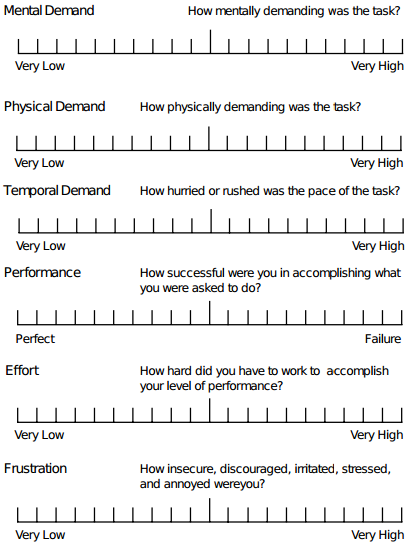
\includegraphics[scale=0.4]{../images/ratingscale.png}
	\caption{NASA TLX Rating Scales}
\end{figure}

After the participants have given a rating on each of the six subscales, they are asked to carry out a pairwise comparison between the subscales to identify their relative importance, in the eyes of the user.

This particular experiment involves asking the user to carry out pairwise comparisons, however, some research has suggested that the exclusion of the pairwise comparisons between subscales can increase experimental validity\cite{tlxinvariance}.

%==============================================================================================
\section{User Interface Evaluation Results}
\label{results}

The results from the user interface evaluation using heuristic evaluation, think-aloud and NASA Task Load Index (TLX) are discussed below.

\subsection{Heuristic Evaluation}
\subsubsection{Visibility of system status}
The system gives users little information about what is going on. For example, on pressing the populate or route buttons, no information is displayed on the screen informing the user that something is happening in the background. As a result, the user could be left wondering whether the button was correctly clicked.

Inclusion of messages on the screen stating what is happening at a particular moment in time would help the users to identify the status of the system. For example, inclusion of a message saying that the system is loading instead of a black screen will inform the user that something is indeed happening. Messages when the user clicks a button confirming that the action is happening and a message that displays on the screen when the evacuation simulation has finished will also increase the user’s awareness of the system status which in turn makes the system more user friendly.

\subsubsection{Match between system and real world}
The arrow keys (up, down, left and right) for camera movement are positioned in a logical order which would be familiar to the majority of users. This allows an easy mapping from real world natural conventions to the system which makes the system easier to use. Non-natural placement of these buttons on the screen would cause confusion in users and lead to frustration.

The system does use the term `navmesh' in the checkbox labelled `show navmesh'. The user is likely to be unfamiliar with this technical term and would thus have to consult the documentation to learn properly what it does. The system should use words and phrases familiar to the user so it would seem appropriate to replace the word `navmesh' with something along the lines of `ship outline' or `wireframe'.

\subsubsection{User control and freedom}
The user has the ability to control the camera manually using the on-screen buttons. The allows the user to view the ship in any way they want. There is also functionality to increase or decrease the speed of the camera and also to select preset camera locations from a drop-down menu which increases the control and freedom the user has. The number of preset camera locations is currently two. This should be expanded to give the user more options.

The user can change the population size from the main screen and a more advanced settings menu allows the user to create categories of people according to various factors. This gives advanced users more freedom in the interactions they make with the system.

\subsubsection{Consistency and standards}
In general, the buttons are labelled well and the user does have to wonder what they do. However, some problems exist in the camera settings part of the main screen. There are two up arrows and two down arrows and their functionality is not made entirely clear to the user. One of the up arrows is to pan up and the other up arrow is to rotate upwards. This should be made clear to the user by either increasing the size of the button and including a meaningful button name, or include the information as text above the buttons on the camera controls panel itself.

\subsubsection{Error prevention}
Some steps have been taken to prevent the users from executing an action which would lead to an error in the system. The evacuate button is grayed out and is only allowed to be clicked by the user when the ship has been successfully populated. By stopping the user from performing this action until it is appropriate, allows the prevention of an illegal system state -- namely evacuating an empty ship.

Error prevention related to the other buttons was overlooked and should be corrected. Other buttons on the main panel of the user interface should also be grayed out when it would not be appropriate to click.

Where there exist fields which can be altered by the user (for example, the population size field) a maximum and minimum value has been defined to prevent the user from entering too high or too low a number. This eliminates the possibility that the system will enter a state which it cannot handle as a result of user input which protects the system from mistakes made by the user.

\subsubsection{Recognition rather than recall}
The main buttons on the user interface are made to be as self explanatory as possible, however one shortfall is the design of the camera location panel. As discussed in the consistency heuristic, it should be made more clear what these buttons actually do. This would remove the need of the user to consult documentation for help and would thus reduce the extent of recall from one dialog to the next.

\subsubsection{Flexibility and efficiency of use}
The system has the ability to cater for more experienced user as mentioned in the user control and freedom heuristic. There exists the ability for the more experienced user to change a variety of properties of the camera such as speed and location. There is also the ability to use the keyboard to navigate around the ship which would allow more experienced users to increase their speed of interaction with the system.

There is, however, no method of allowing the user to tailor frequent actions through the use of accelerators or custom keyboard shortcuts, for example. The addition of such features would increase development time and since the experienced users group is a minority, it would not be in the best interest to develop this feature at this time.

\subsubsection{Aesthetic and minimalist design}
The system has a main screen which includes the most often used actions, and a settings screen which includes extra functionality. This separation allows a less cluttered minimalist view in the main screen which is easier to comprehend for the user. The system had been designed to display elements positioned in a natural way, allowing the user to focus on using the system and not needing to familiarise themselves with the interface for too long.   

\subsubsection{Help users recognize, diagnose and recover from errors}
As mentioned in the prevention of errors heuristic above, some steps have been taken to prevent the user from making errors. However, since not all sections of the interface are removed from use when they are not supposed to be used, it is possible for a user to crash the system by pressing the buttons repeatedly. There are no friendly error messages to tell the user that something has went wrong -- they are presented with a black screen. This leaves the user wondering whether the system is busy in the background carrying out some task, or has crashed.

To resolve this problem, better messages should be displayed on the screen to the user to increase visibility of system status. This would eliminate any confusion from the user when using the system. A reset button should also be implemented as a last resort for the user to click if the system crashes for an undocumented reason. This will ensure robustness in the system and increase the user-friendliness as a whole.

\subsubsection{Help and documentation}
No help or documentation is provided to the user. While the majority of the system is, on the whole, quite intuitive to use, some parts such as the camera controls panel and the advanced settings dialog box would benefit from documentation.

Brief documentation on the basic parts of the interface and what each button does as well as more detailed documentation on the more complex parts of the system should be created to assist the user in using the system and making decisions.

\subsection{Think Aloud}
The Think Aloud evaluation of the user interface was carried out with eight participants. The participants were asked to complete the six tasks listed below and were encouraged to ‘think aloud’ during the evaluation. The participants were observed and notes were taken to allow a discussion of improvements which could be made to the user interface after the evaluation.
\\
\\
\textbf{Tasks}
\begin{enumerate}
\item Set the population size to 50. Populate the ship.
\item Hide the ship frame from view, then show it again.
\item Generate the exit routes for the population.
\item Change the camera angle so you have a bird's eye view of the ship.
\item Evacuate the ship. While the evacuation is taking place, change the camera view to face the exits of the ship.
\item Read out loud the time the simulation took and the number of people evacuated.
\end{enumerate}
A summary of the findings of the Think Aloud evaluation is discussed below. Detailed notes on a per-participant level are included in Appendix C.

\begin{itemize}
\item The visibility of system status was a clear shortfall as indicated by the participants. Particularly in tasks 1, 3 and 5 where buttons which required the user to wait after being pressed, the participant was left guessing whether anything was happening with the system or whether they had done something wrong.
\item The meaning of the camera location buttons was also not as clear as they should have been. Participants had to investigate what the buttons did and clear labelling would have solved this issue.
\item The participants had no difficulty identifying key information such as number of people evacuated and the time taken for the evacuation which confirms that the information is well visible and the labelling is unambiguous.
\item Identification of the completion of the evacuation was most often done by looking at whether anything more was happening in the graphical representation rather than looking at the `remaining people' metric at the right hand side of the interface. It was noted that a pop-up message when the simulation is complete would make this more clear to the user.
\item The terminology used in the user interface must be standardised to remove jargon words such as ‘navmesh’ which would be unclear to the user. Task 2 highlighted that while some users guessed that ‘ship frame’ was equivalent to the ‘navmesh’ in this particular situation, 5 of the 8 participants were confused by the technical language. 
\end{itemize}

\subsection{NASA TLX: Task Load Index}
%\begin{itemize}
%\item Insert graph.
%\item Discuss that there is a low workload in using the system.
%\end{itemize}

\begin{figure}[H]
	\centering
	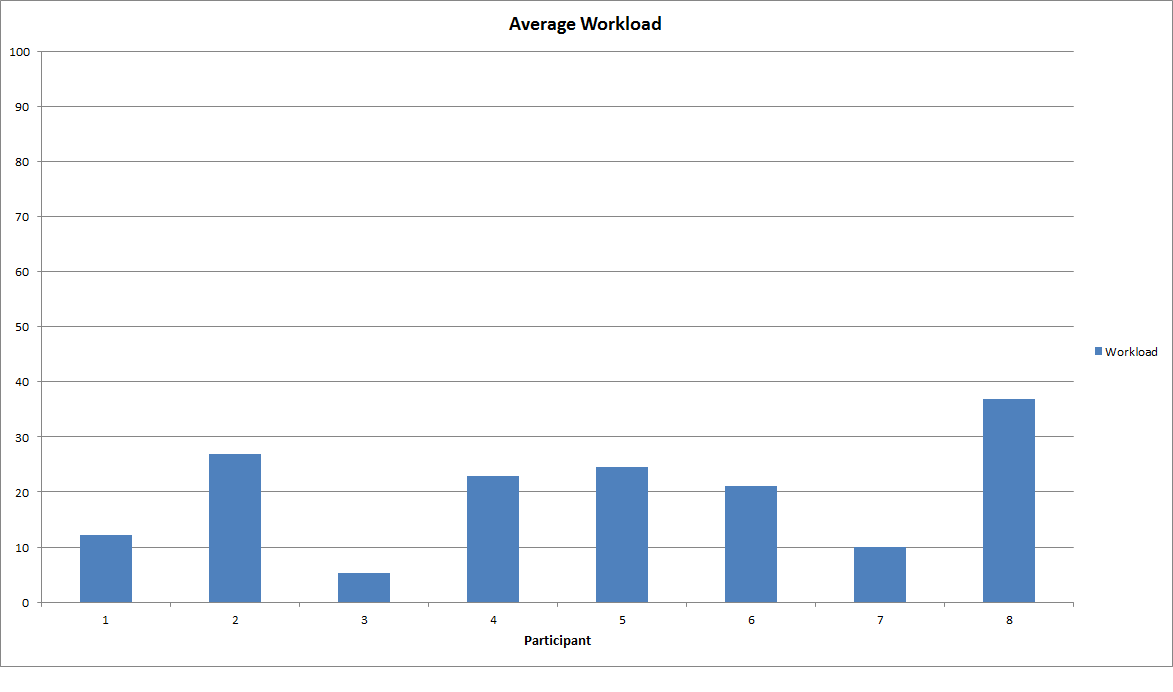
\includegraphics[scale=0.25]{../images/tlxresults.png}
	\caption{Average workload across participants}
\end{figure}

The above image shows the average workload of the eight participants in the experiment, which is calculated based on the ratings and pairwise comparisons given by the participant. It can be seen that the overall workload of each participant is reasonably low and so it can be said that using the system is not demanding. 

%==============================================================================================


%==============================================================================
%\end{document}
 %not complete

%==============================================================================
\chapter{Conclusion}
\label{conclusion}

A great project!

%==============================================================================
\section{Contributions}
\label{contributions}

Here we explain that Lewis Carroll wrote chapter \ref{intro}. John Wayne
was out riding his horse every day and didn't do anything. Marilyn Monroe
was great at getting the requirements specification and coordinating the
writing of the report. Betty Davis did the coding of the kernel of the
project, described in Chapter \ref{impl}.  James Dean handled the
multimedia content of the project.

%==============================================================================
\bibliographystyle{unsrt}
\bibliography{teamL_dissertation_2013}
\end{document}
